\documentclass[11pt]{article}
\usepackage[T1]{fontenc}
\usepackage[utf8]{inputenc}
\usepackage{enumerate}
\usepackage{setspace}
\usepackage{amsmath,amssymb,amsthm}
\usepackage{graphicx}
\usepackage{bbm}
\usepackage[round]{natbib}
\usepackage[nohead]{geometry}
\usepackage[bottom]{footmisc}
\usepackage{indentfirst}
\usepackage{endnotes}
\usepackage{graphicx}%
\usepackage{eurosym}
\usepackage{array}
\usepackage{booktabs}
\usepackage{caption}
\usepackage{subcaption}
\usepackage{rotating}
% \usepackage[hidelinks]{hyperref}
\usepackage{floatrow} %[capposition=top]
\floatsetup{footposition=bottom,capposition=top}
\renewcommand{\labelitemi}{--}
\renewcommand{\labelitemii}{$\bullet$}
\bibliographystyle{chicago}
% \geometry{left=1in,right=1in,top=1.00in,bottom=1.0in}
\let\olditemize\itemize
\renewcommand{\itemize}{
  \olditemize
  \setlength{\itemsep}{-1pt}
}

\begin{document}

\title{French grocery stores\ \\ \ \\(Very preliminary)}
\author{LEI\thanks{e-mail:
\textit{etienne.chamayou@ensae.fr}}\medskip\\{\normalsize CREST and Department of Economics, Ecole Polytechnique }}
\maketitle

\sloppy%

\onehalfspacing

\textbf{Abstract:}

This note provides an overview of French grocery stores in 2014. All the analysis relies on data provided by LSA on hypermarkets, supermarkets, hard discount stores and "drive-through".

\strut

\textbf{Keywords:}

\strut

\textbf{JEL Classification Numbers:} XXX

\pagebreak%
\doublespacing

\section{Introduction}

Data provided by LSA include17,254 French grocery stores. LSA provide three columns regarding the activity of stores over time: an opening date, a closing date and a reopenening date. Stores can thus be considered closed when they have a closing date but no reopening date. According to LSA data, beginning 2014, there were 15,086 hypermarkets, supermarkets, hard discount and "drive-through" stores operating in France.



\section{Overview of store population by type}


\subsection{Surface by type}

Descriptive statistics on surface by type show that grocery stores with a surface between 400 and 2500 $m^2$ are categorized as supermarkets, while those with a surface exceeding 2500 $m^2$ are categorized as hypermarkets. The type "Magasins Populaires" is attributed to stores with a significant surface dedicated to non food products (most of them belong to the same retail chain as will be shown later).

\begin{table}[H]
\caption{Surface in $m^2$ by type of store}
\small

\begin{tabular}{lrrrrrrrrr}
\toprule
{} &     \#Total &    \#Avail. &        Min &        Q05 &        Med &        Avg &        Q95 &        Max &        Cum \\
\midrule
Hypermarkets  &      2,031 &      2,031 &      2,500 &      2,512 &      4,000 &      5,360 &     12,288 &     24,000 & 10,885,500 \\
Supermarkets  &      5,771 &      5,771 &        400 &        406 &      1,200 &      1,286 &      2,346 &      2,499 &  7,422,118 \\
Hard discount &      4,477 &      4,477 &        100 &        318 &        770 &        772 &      1,171 &      2,000 &  3,455,127 \\
\midrule
All           &     12,279 &     12,279 &        100 &        400 &        990 &      1,772 &      6,000 &     24,000 & 21,762,745 \\
\bottomrule
\end{tabular}

\end{table}




\subsection{Number of employees}

\begin{table}[H]
\caption{Number of employees by type of store}
\small

\begin{tabular}{lrrrrrrrrr}
\toprule
{} &     \#Total &    \#Avail. &        Min &        Q05 &        Med &        Avg &        Q95 &        Max &        Cum \\
\midrule
Hypermarkets  &      2,031 &      2,031 &         20 &         45 &        125 &        171 &        450 &      1,000 &    346,928 \\
Supermarkets  &      5,771 &      5,771 &          1 &          6 &         26 &         29 &         65 &        200 &    165,983 \\
Hard discount &      4,477 &      4,477 &          2 &          5 &          9 &         10 &         20 &        151 &     44,267 \\
\midrule
All           &     12,279 &     12,279 &          1 &          5 &         17 &         45 &        200 &      1,000 &    557,178 \\
\bottomrule
\end{tabular}

\end{table}


\subsection{Number of checkouts by type}

\begin{table}[H]
\caption{Number of checkouts by type of store}
\small

\begin{tabular}{lrrrrrrrrr}
\toprule
{} &     \#Total &    \#Avail. &        Min &        Q05 &        Med &        Avg &        Q95 &        Max &        Cum \\
\midrule
Hypermarkets  &      2,031 &      2,030 &          5 &         10 &         19 &         23 &         50 &        358 &     47,307 \\
Supermarkets  &      5,771 &      5,771 &          1 &          3 &          6 &          7 &         12 &         27 &     39,332 \\
Hard discount &      4,477 &      4,476 &          1 &          2 &          4 &          4 &          8 &         42 &     19,495 \\
\midrule
All           &     12,279 &     12,277 &          1 &          2 &          6 &          9 &         26 &        358 &    106,134 \\
\bottomrule
\end{tabular}

\end{table}


\subsection{Size of Parking by type}

\begin{table}[H]
\caption{Size of parking by type of store}
\small

\begin{tabular}{lrrrrrrrrr}
\toprule
{} &     \#Total &    \#Avail. &        Min &        Q05 &        Med &        Avg &        Q95 &        Max &        Cum \\
\midrule
Hypermarkets  &      2,031 &      1,933 &         18 &        170 &        500 &        759 &      2,191 &      7,660 &  1,467,088 \\
Supermarkets  &      5,771 &      4,323 &          2 &         30 &        120 &        135 &        300 &      2,577 &    585,731 \\
Hard discount &      4,477 &      1,509 &          3 &         29 &         73 &         87 &        200 &      1,200 &    131,833 \\
\midrule
All           &     12,279 &      7,765 &          2 &         30 &        140 &        281 &      1,100 &      7,660 &  2,184,652 \\
\bottomrule
\end{tabular}

\end{table}


\subsection{Number of gas pumps}

\begin{table}[H]
\caption{Number of gas pumps by type of store}
\small

\begin{tabular}{lrrrrrrrrr}
\toprule
{} &     \#Total &    \#Avail. &        Min &        Q05 &        Med &        Avg &        Q95 &        Max &        Cum \\
\midrule
Hypermarkets  &      2,031 &      1,786 &          1 &          4 &          7 &          8 &         14 &         26 &     13,956 \\
Supermarkets  &      5,771 &      2,912 &          0 &          2 &          4 &          4 &          7 &         16 &     11,568 \\
Hard discount &      4,477 &        131 &          1 &          2 &          4 &          4 &          6 &         23 &        519 \\
\midrule
All           &     12,279 &      4,829 &          0 &          2 &          4 &          5 &         12 &         26 &     26,043 \\
\bottomrule
\end{tabular}

\end{table}

\section{Overview of competition}

\begin{table}[H]
\caption{Competition at the municipality level}
\small

\begin{tabular}{lrrrrrrrr}
\toprule
{} &      count &       mean &        std &        min &        25\% &        50\% &        75\% &        max \\
\midrule
avail\_surf &  36,253 &  29,958 &  53,296 &   1,027 &  11,516 &  18,319 &  30,173 & 800,164 \\
hhi        &  36,253 &       0.19 &       0.04 &       0.10 &       0.16 &       0.19 &       0.21 &       0.48 \\
CR1        &  36,253 &       0.30 &       0.07 &       0.14 &       0.25 &       0.29 &       0.33 &       0.67 \\
CR2        &  36,253 &       0.51 &       0.08 &       0.28 &       0.45 &       0.51 &       0.56 &       0.87 \\
CR3        &  36,253 &       0.66 &       0.08 &       0.41 &       0.61 &       0.66 &       0.72 &       0.95 \\
All\_dist   &  36,253 &       5.43 &       3.62 &       0.00 &       2.82 &       5.05 &       7.49 &      27.14 \\
H\_dist     &  36,253 &      10.78 &       6.89 &       0.00 &       5.70 &       9.58 &      14.57 &      51.92 \\
S\_dist     &  36,253 &       6.16 &       3.93 &       0.00 &       3.38 &       5.71 &       8.36 &      27.43 \\
X\_dist     &  36,253 &       8.28 &       5.37 &       0.00 &       4.37 &       7.44 &      11.25 &      40.71 \\
\bottomrule
\end{tabular}

\end{table}

\section{Stores and surface by group and chain}

This section focuses on hypermarkets, supermarkets and hard discount stores (exclude?). "Drive-through" are thus left aside.

\subsection{Stores and surface by group}

The following table shows the number of hypermarkets, supermarkets and hard discount stores operated by the main grocery store groups in France.

\begin{table}[H]
\caption{Type of store and surface by retail group}
\footnotesize
\setlength{\tabcolsep}{2pt}

\begin{tabular}{l|rrrr|rrrr|rrr}
\toprule
{}             & \multicolumn{4}{c|}{Nb} &   \multicolumn{4}{c|}{Cum Surf. (mil $m^2$)}   &   \multicolumn{3}{c}{Avg. Surf. ($m^2$)}\\
{}             &        All &  Hyp       &        Sup &       Dis  &      All   & Hyp        &        Sup &        Dis &      Hyp   &       Sup  &    Dis \\
\midrule
CARREFOUR      &      2,560 &        372 &      1,369 &        819 &       4.81 &       2.52 &       1.69 &       0.59 &      6,786 &      1,237 &        720 \\
\%             &        100 &         15 &         53 &         32 &        100 &         53 &         35 &         12 &            &            &            \\
MOUSQUETAIRES  &      2,140 &        348 &      1,464 &        328 &       3.58 &       1.10 &       2.23 &       0.24 &      3,173 &      1,523 &        746 \\
\%             &        100 &         16 &         68 &         15 &        100 &         31 &         62 &          7 &            &            &            \\
CASINO         &      2,044 &        216 &      1,162 &        666 &       2.92 &       1.14 &       1.19 &       0.59 &      5,269 &      1,024 &        883 \\
\%             &        100 &         11 &         57 &         33 &        100 &         39 &         41 &         20 &            &            &            \\
LIDL           &      1,522 &          0 &          0 &      1,522 &       1.25 &       0.00 &       0.00 &       1.25 &            &            &        824 \\
\%             &        100 &          0 &          0 &        100 &        100 &          0 &          0 &        100 &            &            &            \\
SYSTEME U      &      1,059 &        337 &        722 &          0 &       2.28 &       1.21 &       1.07 &       0.00 &      3,593 &      1,482 &            \\
\%             &        100 &         32 &         68 &          0 &        100 &         53 &         47 &          0 &            &            &            \\
ALDI           &        917 &          0 &          0 &        917 &       0.64 &       0.00 &       0.00 &       0.64 &            &            &        698 \\
\%             &        100 &          0 &          0 &        100 &        100 &          0 &          0 &        100 &            &            &            \\
LECLERC        &        626 &        522 &        104 &          0 &       2.98 &       2.82 &       0.15 &       0.00 &      5,408 &      1,463 &            \\
\%             &        100 &         83 &         17 &          0 &        100 &         95 &          5 &          0 &            &            &            \\
AUCHAN         &        565 &        159 &        406 &          0 &       2.00 &       1.44 &       0.56 &       0.00 &      9,074 &      1,380 &            \\
\%             &        100 &         28 &         72 &          0 &        100 &         72 &         28 &          0 &            &            &            \\
LOUIS DELHAIZE &        201 &         69 &        132 &          0 &       0.80 &       0.60 &       0.20 &       0.00 &      8,693 &      1,536 &            \\
\%             &        100 &         34 &         66 &          0 &        100 &         75 &         25 &          0 &            &            &            \\
DIAPAR         &        116 &          0 &        116 &          0 &       0.06 &       0.00 &       0.06 &       0.00 &            &        533 &            \\
\%             &        100 &          0 &        100 &          0 &        100 &          0 &        100 &          0 &            &            &            \\
COLRUYT        &        110 &          0 &        110 &          0 &       0.09 &       0.00 &       0.09 &       0.00 &            &        837 &            \\
\%             &        100 &          0 &        100 &          0 &        100 &          0 &        100 &          0 &            &            &            \\
AUTRE          &        419 &          8 &        186 &        225 &       0.35 &       0.04 &       0.17 &       0.14 &      5,307 &        917 &        615 \\
\%             &        100 &          2 &         44 &         54 &        100 &         12 &         49 &         39 &            &            &            \\

\midrule
ALL            &     12,279 &      2,031 &      5,771 &      4,477 &      21.76 &      10.89 &       7.42 &       3.46 &      5,360 &      1,286 &        772 \\
\%             &        100 &         17 &         47 &         36 &        100 &         50 &         34 &         16 &            &            &            \\
\bottomrule
\end{tabular}

\end{table}

\subsection{Stores and surface by group and chain}

Except for Aldi and Lidl, stores are subdivided in retail chains based on criteria such as the size or the location (city center, suburb, countryside etc.).

\subsubsection{Carrefour}

\begin{table}[H]
\footnotesize
\setlength{\tabcolsep}{2pt}

\begin{tabular}{lrrrrrrrrr}
\toprule
All Carrefour &       \#Tot &       \#Hyp &       \#Sup &       \#Dis &     Avg S. &     Med S. &     Min S. &     Max S. &     Cum S. \\
\midrule
DIA \%             &        819 &          0 &          0 &        819 &        720 &        782 &        215 &      1,280 &       0.59 \\
CARREFOUR MARKET  &        801 &        114 &        687 &          0 &      1,894 &      1,800 &        654 &      5,600 &       1.52 \\
CARREFOUR CONTACT &        402 &          0 &        402 &          0 &        682 &        670 &        400 &      1,800 &       0.27 \\
CARREFOUR         &        221 &        221 &          0 &          0 &      9,319 &      9,000 &      2,500 &     24,000 &       2.06 \\
CARREFOUR CITY    &        123 &          0 &        123 &          0 &        504 &        450 &        400 &        800 &       0.06 \\
MARKET            &        121 &         37 &         84 &          0 &      2,204 &      2,200 &        722 &      4,500 &       0.27 \\
SHOPI             &         34 &          0 &         34 &          0 &        573 &        500 &        400 &        870 &       0.02 \\
CARREFOUR EXPRESS &         21 &          0 &         21 &          0 &        475 &        460 &        400 &        750 &       0.01 \\
CARREFOUR AUTRE   &         18 &          0 &         18 &          0 &        482 &        450 &        400 &        821 &       0.01 \\
\bottomrule
\multicolumn{10}{l}{\footnotesize Surfaces are in $m^2$ except for Cum S. which is in million $m^2$} \\
\end{tabular}

\end{table}

\begin{table}[H]
\footnotesize
\setlength{\tabcolsep}{2pt}

\begin{tabular}{lrrrrrrrrr}
\toprule
Independent Carrefour &       \#Tot &       \#Hyp &       \#Sup &       \#Dis &     Avg S. &     Med S. &     Min S. &     Max S. &     Cum S. \\
\midrule
CARREFOUR CONTACT &        398 &          0 &        398 &          0 &        683 &        670 &        400 &      1,800 &       0.27 \\
CARREFOUR MARKET  &        388 &         48 &        340 &          0 &      1,807 &      1,700 &        800 &      4,800 &       0.70 \\
CARREFOUR CITY    &        123 &          0 &        123 &          0 &        504 &        450 &        400 &        800 &       0.06 \\
DIA \%             &         68 &          0 &          0 &         68 &        769 &        820 &        243 &      1,200 &       0.05 \\
SHOPI             &         34 &          0 &         34 &          0 &        573 &        500 &        400 &        870 &       0.02 \\
CARREFOUR EXPRESS &         21 &          0 &         21 &          0 &        475 &        460 &        400 &        750 &       0.01 \\
CARREFOUR AUTRE   &         18 &          0 &         18 &          0 &        482 &        450 &        400 &        821 &       0.01 \\
MARKET            &         13 &          1 &         12 &          0 &      1,744 &      1,800 &        900 &      2,680 &       0.02 \\
CARREFOUR         &         10 &         10 &          0 &          0 &      7,796 &      7,246 &      5,006 &     10,842 &       0.08 \\
\bottomrule
\multicolumn{10}{l}{\footnotesize Surfaces are in $m^2$ except for Cum S. which is in million $m^2$} \\
\end{tabular}

\end{table}

As of September 2014, Carrefour listed the following chains on its website: "Carrefour", "Carrefour market" (created in 2007 to replace "Champion"), "Carrefour contact" (created in 2008 for stores located in rural areas or in the periphery of cities), "Carrefour city" (created in 2009 for stores located in city centers, opening 6/7 days 7h-22h or 23h), "Carrefour montagne" (crated in 2009 for small stores located in the mountains), "Carrefour express" (created in 2007 for small stores, difference with "city" and "contact" is not clear) and "Market" (created in 2012, includes virtually all ex-"Hyper champion").

\subsubsection{Casino}

\begin{table}[H]
\footnotesize
\setlength{\tabcolsep}{2pt}

\begin{tabular}{lrrrrrrrrr}
\toprule
All Casino &       \#Tot &       \#Hyp &       \#Sup &       \#Dis &     Avg S. &     Med S. &     Min S. &     Max S. &     Cum S. \\
\midrule
LEADER PRICE &        666 &          0 &          0 &        666 &        883 &        880 &        100 &      2,000 &       0.59 \\
FRANPRIX     &        448 &          0 &        448 &          0 &        608 &        500 &        400 &      2,400 &       0.27 \\
CASINO       &        341 &         16 &        325 &          0 &      1,513 &      1,500 &        415 &      3,000 &       0.52 \\
MONOPRIX     &        296 &         60 &        236 &          0 &      1,792 &      1,656 &        402 &      5,154 &       0.53 \\
SPAR         &        113 &          0 &        113 &          0 &        560 &        550 &        400 &      1,200 &       0.06 \\
GEANT CASINO &        103 &        103 &          0 &          0 &      7,668 &      7,600 &      3,800 &     17,112 &       0.79 \\
HYPER CASINO &         44 &         37 &          7 &          0 &      3,138 &      2,800 &      2,160 &      5,950 &       0.14 \\
MONOP'       &         19 &          0 &         19 &          0 &        565 &        515 &        400 &      1,000 &       0.01 \\
CASINO AUTRE &         14 &          0 &         14 &          0 &        518 &        520 &        400 &        698 &       0.01 \\
\bottomrule
\multicolumn{10}{l}{\footnotesize Surfaces are in $m^2$ except for Cum S. which is in million $m^2$} \\
\end{tabular}

\end{table}

\begin{table}[H]
\footnotesize
\setlength{\tabcolsep}{2pt}

\begin{tabular}{lrrrrrrrrr}
\toprule
Independent Casino &       \#Tot &       \#Hyp &       \#Sup &       \#Dis &     Avg S. &     Med S. &     Min S. &     Max S. &     Cum S. \\
\midrule
LEADER PRICE &        489 &          0 &          0 &        489 &        886 &        896 &        100 &      2,000 &       0.43 \\
FRANPRIX     &        444 &          0 &        444 &          0 &        607 &        500 &        400 &      2,400 &       0.27 \\
SPAR         &         72 &          0 &         72 &          0 &        566 &        550 &        400 &      1,200 &       0.04 \\
CASINO       &         41 &          0 &         41 &          0 &      1,192 &      1,050 &        476 &      1,900 &       0.05 \\
MONOPRIX     &         35 &          4 &         31 &          0 &      1,476 &      1,421 &        442 &      3,371 &       0.05 \\
MONOP'       &          9 &          0 &          9 &          0 &        606 &        500 &        450 &      1,000 &       0.01 \\
CASINO AUTRE &          4 &          0 &          4 &          0 &        445 &        440 &        400 &        500 &       0.00 \\
\bottomrule
\multicolumn{10}{l}{\footnotesize Surfaces are in $m^2$ except for Cum S. which is in million $m^2$} \\
\end{tabular}

\end{table}

\subsubsection{Les Mousquetaires}

\begin{table}[H]
\footnotesize
\setlength{\tabcolsep}{2pt}

\begin{tabular}{lrrrrrrrrr}
\toprule
{} &       \#Tot &       \#Hyp &       \#Sup &       \#Dis &     Avg S. &     Med S. &     Min S. &     Max S. &     Cum S. \\
\midrule
INTERMARCHE SUPER   &      1,362 &        252 &      1,110 &          0 &      1,947 &      1,950 &        499 &      4,100 &       2.65 \\
NETTO               &        328 &          0 &          0 &        328 &        746 &        704 &        100 &      1,780 &       0.24 \\
INTERMARCHE CONTACT &        312 &          0 &        312 &          0 &        804 &        800 &        400 &      1,500 &       0.25 \\
INTERMARCHE HYPER   &         96 &         96 &          0 &          0 &      4,119 &      4,000 &      2,800 &      6,710 &       0.40 \\
INTERMARCHE EXPRESS &         37 &          0 &         37 &          0 &        878 &        928 &        400 &      1,340 &       0.03 \\
INTERMARCHE AUTRE   &          5 &          0 &          5 &          0 &        642 &        620 &        400 &        988 &       0.00 \\
\bottomrule
\multicolumn{10}{l}{\footnotesize Surfaces are in $m^2$ except for Cum S. which is in million $m^2$} \\
\end{tabular}

\end{table}

\begin{table}[H]
\footnotesize
\setlength{\tabcolsep}{2pt}

\begin{tabular}{lrrrrrrrrr}
\toprule
{} &       \#Tot &       \#Hyp &       \#Sup &       \#Dis &     Avg S. &     Med S. &     Min S. &     Max S. &     Cum S. \\
\midrule
INTERMARCHE SUPER   &      1,361 &        252 &      1,109 &          0 &      1,947 &      1,950 &        499 &      4,100 &       2.65 \\
NETTO               &        328 &          0 &          0 &        328 &        746 &        704 &        100 &      1,780 &       0.24 \\
INTERMARCHE CONTACT &        312 &          0 &        312 &          0 &        804 &        800 &        400 &      1,500 &       0.25 \\
INTERMARCHE HYPER   &         96 &         96 &          0 &          0 &      4,119 &      4,000 &      2,800 &      6,710 &       0.40 \\
INTERMARCHE EXPRESS &         37 &          0 &         37 &          0 &        878 &        928 &        400 &      1,340 &       0.03 \\
INTERMARCHE AUTRE   &          5 &          0 &          5 &          0 &        642 &        620 &        400 &        988 &       0.00 \\
\bottomrule
\multicolumn{10}{l}{\footnotesize Surfaces are in $m^2$ except for Cum S. which is in million $m^2$} \\
\end{tabular}

\end{table}

\subsubsection{Système U}

\begin{table}[H]
\footnotesize
\setlength{\tabcolsep}{2pt}

\begin{tabular}{lrrrrrrrrr}
\toprule
{} &       \#Tot &       \#Hyp &       \#Sup &       \#Dis &     Avg S. &     Med S. &     Min S. &     Max S. &     Cum S. \\
\midrule
SUPER U   &        729 &        272 &        457 &          0 &      2,339 &      2,273 &        700 &      5,200 &  1,705,104 \\
U EXPRESS &        230 &          1 &        229 &          0 &        862 &        802 &        400 &      2,854 &    198,164 \\
HYPER U   &         64 &         64 &          0 &          0 &      5,621 &      5,310 &      3,003 &     11,750 &    359,726 \\
UTILE     &         32 &          0 &         32 &          0 &        486 &        455 &        400 &        700 &     15,556 \\
MARCHE U  &          4 &          0 &          4 &          0 &        626 &        550 &        450 &        956 &      2,506 \\
\bottomrule
\end{tabular}

\end{table}


\subsubsection{Leclerc}

\begin{table}[H]
\footnotesize
\setlength{\tabcolsep}{2pt}

\begin{tabular}{lrrrrrrrrrr}
\toprule
LECLERC &       \#Tot &       \#Hyp &       \#Sup &       \#Dis &        \#MP &     Avg S. &     Med S. &     Min S. &     Max S. &     Cum S. \\
\midrule
CENTRE E.LECLERC &        581 &        526 &         55 &          0 &          0 &       5063 &       4709 &        826 &      15600 &    2941426 \\
LECLERC EXPRESS  &         71 &          1 &         70 &          0 &          0 &       1059 &        995 &        400 &       3500 &      75201 \\
\bottomrule
\end{tabular}

\end{table}



\subsubsection{Auchan}

\begin{table}[H]
\footnotesize
\setlength{\tabcolsep}{2pt}

\begin{tabular}{lrrrrrrrrr}
\toprule
{} &       \#Tot &       \#Hyp &       \#Sup &       \#Dis &     Avg S. &     Med S. &     Min S. &     Max S. &     Cum S. \\
\midrule
SIMPLY MARKET       &        304 &         16 &        288 &          0 &      1,577 &      1,523 &        605 &      3,624 &    479,471 \\
AUCHAN              &        135 &        135 &          0 &          0 &     10,102 &      9,985 &      2,800 &     19,700 &  1,363,828 \\
ATAC                &         77 &          0 &         77 &          0 &      1,339 &      1,200 &        700 &      2,450 &    103,135 \\
LES HALLES D'AUCHAN &          7 &          7 &          0 &          0 &      4,124 &      4,000 &      2,800 &      5,650 &     28,870 \\
AUCHAN CITY         &          1 &          1 &          0 &          0 &      4,000 &      4,000 &      4,000 &      4,000 &      4,000 \\
AUCHAN AUTRE        &         41 &          0 &         41 &          0 &        573 &        550 &        400 &        900 &     23,481 \\
\bottomrule
\end{tabular}

\end{table}


\subsubsection{Louis Delhaize}

\begin{table}[H]
\footnotesize
\setlength{\tabcolsep}{2pt}

\begin{tabular}{lrrrrrrrrrr}
\toprule
LOUIS DELHAIZE &       \#Tot &       \#Hyp &       \#Sup &       \#Dis &        \#MP &     Avg S. &     Med S. &     Min S. &     Max S. &     Cum S. \\
\midrule
SUPERMARCHE MATCH &        144 &         11 &        133 &          0 &          0 &       1621 &       1621 &        450 &       2900 &     233353 \\
CORA              &         59 &         59 &          0 &          0 &          0 &       9725 &       9385 &       2500 &      15500 &     573763 \\
\bottomrule
\end{tabular}*
\end{table}


\subsubsection{Diapar}

\begin{table}[H]
\footnotesize
\setlength{\tabcolsep}{2pt}

\begin{tabular}{lrrrrrrrrr}
\toprule
{} &       \#Tot &       \#Hyp &       \#Sup &       \#Dis &     Avg S. &     Med S. &     Min S. &     Max S. &     Cum S. \\
\midrule
G 20         &         95 &          0 &         95 &          0 &        546 &        420 &        400 &      1,200 &     51,895 \\
AUTRE DIAPAR &         21 &          0 &         21 &          0 &        473 &        400 &        400 &        828 &      9,928 \\
\bottomrule
\end{tabular}

\end{table}


\subsubsection{Colruyt}

\begin{table}[H]
\footnotesize
\setlength{\tabcolsep}{2pt}

\begin{tabular}{lrrrrrrrrr}
\toprule
{} &       \#Tot &       \#Hyp &       \#Sup &       \#Dis &     Avg S. &     Med S. &     Min S. &     Max S. &     Cum S. \\
\midrule
COLRUYT    &         69 &          0 &         69 &          0 &      1,002 &        990 &        630 &      1,700 &     69,149 \\
COCCINELLE &         41 &          0 &         41 &          0 &        558 &        500 &        400 &      1,200 &     22,874 \\
\bottomrule
\end{tabular}

\end{table}

\section{Store locations}

The following section offers a brief overview of groups' store locations across France. "Drive-through" is not included.

\subsection{Distribution of stores across regions by retail group}


\begin{table}[H]
\caption{Percentage of stores by region within each group}
\footnotesize
\setlength{\tabcolsep}{2pt}

\begin{tabular}{lrrrrrrrrrrrrr}
\toprule
{} &      CARR. &      CASI. &      MOUS. &       LIDL &      SYS.U &       ALDI &      LECL. &      AUCH. &       L.D. &      DIAP. &      COLR. &       OTH. &       TOT. \\
\midrule
Ile-de-France        &         18 &         36 &          6 &         11 &          5 &          6 &          8 &         23 &          3 &         62 &          3 &          5 &         15 \\
Rhone-Alpes          &         11 &         11 &          9 &          8 &          8 &          5 &          6 &          6 &          0 &          0 &          4 &          8 &          9 \\
PACA                 &          8 &         11 &          7 &          7 &          6 &          6 &          6 &          4 &          0 &          0 &          0 &          4 &          7 \\
Nord-Pas-de-Calais   &         11 &          2 &          5 &          9 &          2 &         16 &          4 &          6 &         29 &          1 &          5 &          1 &          7 \\
Bretagne             &          4 &          4 &          9 &          6 &         12 &          2 &         10 &          0 &          1 &          4 &          3 &          1 &          6 \\
Aquitaine            &          5 &          5 &          8 &          6 &          5 &          3 &          9 &          4 &          0 &          0 &          2 &          7 &          6 \\
Pays de la Loire     &          4 &          2 &          5 &          6 &         17 &          4 &          8 &          1 &          0 &         10 &          4 &          3 &          5 \\
Midi-Pyrenees        &          4 &          5 &          8 &          5 &          4 &          5 &          5 &          2 &          0 &          1 &          0 &          3 &          5 \\
Languedoc-Roussillon &          4 &          5 &          6 &          6 &          5 &          4 &          2 &          2 &          0 &          5 &          0 &          1 &          4 \\
Lorraine             &          2 &          2 &          3 &          7 &          3 &         10 &          4 &          4 &         31 &          1 &         15 &         11 &          4 \\
Centre               &          4 &          2 &          5 &          4 &          6 &          4 &          5 &          7 &          1 &          7 &          7 &          3 &          4 \\
Picardie             &          4 &          2 &          4 &          3 &          1 &          6 &          4 &          4 &          6 &          2 &          3 &          5 &          3 \\
Bourgogne            &          2 &          2 &          4 &          2 &          1 &          5 &          4 &         15 &          1 &          0 &         12 &          4 &          3 \\
Haute-Normandie      &          4 &          1 &          3 &          3 &          3 &          3 &          3 &          2 &          0 &          0 &          2 &         11 &          3 \\
Alsace               &          1 &          1 &          1 &          4 &          5 &          3 &          7 &          6 &         16 &          0 &          1 &         15 &          3 \\
Poitou-Charentes     &          1 &          2 &          4 &          3 &          7 &          1 &          5 &          2 &          0 &          1 &          1 &          2 &          3 \\
Basse-Normandie      &          4 &          1 &          2 &          3 &          4 &          2 &          3 &          1 &          0 &          3 &          5 &          5 &          3 \\
Champagne-Ardenne    &          2 &          2 &          3 &          2 &          1 &          5 &          4 &          2 &          4 &          1 &          4 &          2 &          2 \\
Franche-Comte        &          1 &          2 &          2 &          2 &          3 &          4 &          1 &          4 &          3 &          0 &         27 &          3 &          2 \\
Auvergne             &          2 &          2 &          3 &          2 &          1 &          3 &          2 &          4 &          1 &          0 &          3 &          3 &          2 \\
Limousin             &          1 &          2 &          2 &          1 &          2 &          2 &          1 &          1 &          0 &          2 &          0 &          1 &          2 \\
TOT.                 &        100 &        100 &        100 &        100 &        100 &        100 &        100 &        100 &        100 &        100 &        100 &        100 &        100 \\
\bottomrule
\end{tabular}

\end{table}

\begin{table}[H]
\caption{Percentage of surface by region within each group}
\footnotesize
\setlength{\tabcolsep}{2pt}

\begin{tabular}{lrrrrrrrrrrrrr}
\toprule
{} &      CARR. &      CASI. &      MOUS. &       LIDL &      SYS.U &       ALDI &      LECL. &      AUCH. &       L.D. &      DIAP. &      COLR. &       OTH. &       TOT. \\
\midrule
Ile-de-France        &         19 &         26 &          6 &         12 &          4 &          6 &          9 &         22 &          7 &         59 &          3 &          8 &         14 \\
Rhone-Alpes          &         12 &         13 &          9 &          8 &          7 &          5 &          6 &          6 &          1 &          0 &          4 &         13 &          9 \\
PACA                 &          8 &         13 &          6 &          7 &          4 &          6 &          5 &          7 &          0 &          0 &          0 &          5 &          7 \\
Nord-Pas-de-Calais   &          9 &          1 &          5 &          9 &          1 &         17 &          4 &         13 &         19 &          1 &          3 &          1 &          7 \\
Pays de la Loire     &          4 &          3 &          5 &          5 &         21 &          4 &         10 &          3 &          0 &         10 &          3 &          3 &          6 \\
Bretagne             &          5 &          5 &          8 &          6 &         12 &          2 &          8 &          0 &          2 &          5 &          2 &          1 &          6 \\
Aquitaine            &          5 &          6 &          8 &          6 &          5 &          3 &          9 &          5 &          0 &          0 &          2 &          6 &          6 \\
Midi-Pyrenees        &          4 &          5 &          7 &          5 &          4 &          5 &          6 &          2 &          0 &          1 &          0 &          2 &          5 \\
Centre               &          4 &          3 &          5 &          4 &          6 &          4 &          5 &          6 &          2 &          7 &          7 &          3 &          5 \\
Lorraine             &          2 &          1 &          4 &          7 &          3 &         10 &          5 &          5 &         27 &          1 &         20 &         11 &          5 \\
Languedoc-Roussillon &          5 &          6 &          7 &          6 &          5 &          4 &          2 &          3 &          1 &          5 &          0 &          1 &          4 \\
Picardie             &          3 &          2 &          5 &          3 &          1 &          6 &          4 &          6 &          6 &          3 &          2 &          4 &          4 \\
Bourgogne            &          3 &          3 &          4 &          2 &          1 &          5 &          3 &          7 &          2 &          0 &         12 &          4 &          3 \\
Poitou-Charentes     &          1 &          2 &          5 &          3 &          7 &          1 &          5 &          2 &          0 &          1 &          1 &          2 &          3 \\
Alsace               &          1 &          1 &          1 &          3 &          5 &          3 &          5 &          4 &         14 &          0 &          1 &         15 &          3 \\
Haute-Normandie      &          4 &          1 &          3 &          3 &          3 &          3 &          3 &          3 &          1 &          0 &          1 &          8 &          3 \\
Basse-Normandie      &          4 &          1 &          3 &          3 &          3 &          2 &          3 &          1 &          1 &          5 &          3 &          4 &          3 \\
Champagne-Ardenne    &          3 &          2 &          3 &          2 &          1 &          5 &          4 &          1 &          7 &          1 &          4 &          2 &          3 \\
Franche-Comte        &          1 &          3 &          2 &          2 &          4 &          4 &          1 &          2 &          4 &          0 &         30 &          3 &          2 \\
Auvergne             &          3 &          2 &          3 &          2 &          1 &          3 &          1 &          3 &          2 &          0 &          2 &          3 &          2 \\
Limousin             &          1 &          2 &          2 &          1 &          2 &          2 &          1 &          1 &          1 &          2 &          0 &          1 &          1 \\
TOT.                 &        100 &        100 &        100 &        100 &        100 &        100 &        100 &        100 &        100 &        100 &        100 &        100 &        100 \\
\bottomrule
\end{tabular}

\end{table}

\subsection{Presence of retail groups within each region}

The following tables provide an overview of the market power of each group by region

\begin{table}[H]
\caption{Percentage of stores operated by each group in each region}
\footnotesize
\setlength{\tabcolsep}{2pt}

\begin{tabular}{lrrrrrrrrrrrrr}
\toprule
{} &      CARR. &      CASI. &      MOUS. &       LIDL &      SYS.U &       ALDI &      LECL. &      AUCH. &       L.D. &      DIAP. &      COLR. &       OTH. &       TOT. \\
\midrule
Ile-de-France        &         24 &         39 &          7 &          9 &          3 &          3 &          3 &          7 &          0 &          4 &          0 &          1 &        100 \\
Rhone-Alpes          &         27 &         21 &         19 &         11 &          8 &          4 &          4 &          3 &          0 &          0 &          0 &          3 &        100 \\
PACA                 &         24 &         26 &         17 &         12 &          7 &          6 &          4 &          2 &          0 &          0 &          0 &          2 &        100 \\
Nord-Pas-de-Calais   &         34 &          4 &         12 &         16 &          2 &         17 &          3 &          4 &          7 &          0 &          1 &          0 &        100 \\
Bretagne             &         17 &         11 &         27 &         14 &         18 &          3 &          9 &          0 &          0 &          1 &          0 &          0 &        100 \\
Aquitaine            &         18 &         15 &         25 &         14 &          7 &          4 &          9 &          4 &          0 &          0 &          0 &          4 &        100 \\
Pays de la Loire     &         16 &          7 &         17 &         14 &         28 &          5 &          7 &          1 &          0 &          2 &          1 &          2 &        100 \\
Midi-Pyrenees        &         19 &         16 &         27 &         13 &          7 &          8 &          6 &          2 &          0 &          0 &          0 &          2 &        100 \\
Languedoc-Roussillon &         20 &         17 &         25 &         16 &         10 &          6 &          2 &          2 &          0 &          1 &          0 &          1 &        100 \\
Lorraine             &         10 &          6 &         13 &         18 &          5 &         16 &          5 &          4 &         11 &          0 &          3 &          9 &        100 \\
Centre               &         20 &          9 &         21 &         11 &         12 &          7 &          6 &          8 &          0 &          2 &          2 &          2 &        100 \\
Picardie             &         26 &          7 &         20 &         11 &          3 &         12 &          6 &          6 &          3 &          0 &          1 &          5 &        100 \\
Bourgogne            &         12 &         12 &         19 &          9 &          4 &         11 &          5 &         20 &          0 &          0 &          3 &          4 &        100 \\
Haute-Normandie      &         27 &          7 &         15 &         11 &          9 &          8 &          5 &          4 &          0 &          0 &          1 &         13 &        100 \\
Alsace               &          4 &          3 &          7 &         15 &         14 &          9 &         12 &         10 &          9 &          0 &          0 &         18 &        100 \\
Poitou-Charentes     &         10 &         13 &         26 &         13 &         22 &          3 &          9 &          3 &          0 &          0 &          0 &          3 &        100 \\
Basse-Normandie      &         29 &          5 &         15 &         14 &         12 &          7 &          6 &          2 &          0 &          1 &          2 &          7 &        100 \\
Champagne-Ardenne    &         19 &         12 &         21 &         12 &          2 &         16 &          7 &          3 &          3 &          0 &          1 &          2 &        100 \\
Franche-Comte        &         11 &         10 &         16 &         12 &         12 &         11 &          3 &          7 &          2 &          0 &         10 &          4 &        100 \\
Auvergne             &         22 &         12 &         23 &         11 &          4 &          9 &          4 &          9 &          1 &          0 &          1 &          4 &        100 \\
Limousin             &         15 &         20 &         24 &          9 &         13 &          7 &          4 &          3 &          1 &          1 &          0 &          3 &        100 \\
TOT.                 &         21 &         17 &         17 &         12 &          9 &          7 &          5 &          5 &          2 &          1 &          1 &          3 &        100 \\
\bottomrule
\end{tabular}

\end{table}

\begin{table}[H]
\caption{Percentage of surface operated by each group in each region}
\footnotesize
\setlength{\tabcolsep}{2pt}

\begin{tabular}{lrrrrrrrrrrrrr}
\toprule
{} &      CARR. &      CASI. &      MOUS. &       LIDL &      SYS.U &       ALDI &      LECL. &      AUCH. &       L.D. &      DIAP. &      COLR. &       OTH. &       TOT. \\
\midrule
Ile-de-France        &         30 &         25 &          7 &          5 &          3 &          1 &          9 &         14 &          2 &          1 &          0 &          1 &        100 \\
Rhone-Alpes          &         30 &         19 &         17 &          5 &          8 &          2 &         10 &          6 &          0 &          0 &          0 &          2 &        100 \\
PACA                 &         26 &         26 &         15 &          6 &          6 &          2 &          9 &          9 &          0 &          0 &          0 &          1 &        100 \\
Nord-Pas-de-Calais   &         31 &          3 &         12 &          8 &          2 &          7 &          8 &         18 &         11 &          0 &          0 &          0 &        100 \\
Pays de la Loire     &         14 &          6 &         13 &          5 &         35 &          2 &         21 &          4 &          0 &          0 &          0 &          1 &        100 \\
Bretagne             &         18 &         11 &         22 &          6 &         22 &          1 &         18 &          0 &          1 &          0 &          0 &          0 &        100 \\
Aquitaine            &         18 &         13 &         22 &          6 &          8 &          2 &         21 &          8 &          0 &          0 &          0 &          2 &        100 \\
Midi-Pyrenees        &         21 &         15 &         24 &          6 &          9 &          3 &         17 &          5 &          0 &          0 &          0 &          1 &        100 \\
Centre               &         21 &          8 &         18 &          5 &         14 &          3 &         15 &         12 &          2 &          0 &          1 &          1 &        100 \\
Lorraine             &          8 &          4 &         14 &          8 &          7 &          6 &         16 &          9 &         22 &          0 &          2 &          4 &        100 \\
Languedoc-Roussillon &         24 &         17 &         25 &          8 &         11 &          3 &          6 &          6 &          1 &          0 &          0 &          0 &        100 \\
Picardie             &         21 &          6 &         22 &          5 &          4 &          5 &         14 &         15 &          6 &          0 &          0 &          2 &        100 \\
Bourgogne            &         19 &         14 &         19 &          4 &          4 &          4 &         13 &         18 &          2 &          0 &          2 &          2 &        100 \\
Poitou-Charentes     &          8 &         10 &         24 &          5 &         23 &          1 &         21 &          7 &          0 &          0 &          0 &          1 &        100 \\
Alsace               &          4 &          3 &          6 &          6 &         17 &          3 &         22 &         13 &         17 &          0 &          0 &          8 &        100 \\
Haute-Normandie      &         29 &          4 &         18 &          5 &         11 &          3 &         15 &          9 &          1 &          0 &          0 &          4 &        100 \\
Basse-Normandie      &         31 &          5 &         17 &          6 &         13 &          2 &         18 &          3 &          2 &          1 &          0 &          3 &        100 \\
Champagne-Ardenne    &         23 &          9 &         18 &          5 &          2 &          6 &         22 &          2 &         10 &          0 &          1 &          1 &        100 \\
Franche-Comte        &         10 &         16 &         17 &          5 &         17 &          5 &          9 &          7 &          7 &          0 &          6 &          2 &        100 \\
Auvergne             &         26 &         13 &         19 &          5 &          4 &          4 &          9 &         13 &          4 &          0 &          0 &          2 &        100 \\
Limousin             &         19 &         16 &         22 &          4 &         16 &          4 &         11 &          4 &          4 &          0 &          0 &          2 &        100 \\
TOT.                 &         22 &         13 &         16 &          6 &         10 &          3 &         14 &          9 &          4 &          0 &          0 &          2 &        100 \\
\bottomrule
\end{tabular}

\end{table}

\subsection{Group market power by region}

\begin{table}[H]
\caption{Percentage of surface operated by each group in each region}
\footnotesize
\setlength{\tabcolsep}{2pt}

\begin{tabular}{lrrrrrrrrrr}
\toprule
{} &      CR1\_n &      CR2\_n &      CR3\_n &      CR4\_n &      CR1\_s &      CR2\_s &      CR3\_s &      CR4\_s &      HHI\_n &      HHI\_s \\
\midrule
Alsace               &         15 &         29 &         41 &         50 &         22 &         39 &         56 &         69 &       0.09 &       0.14 \\
Aquitaine            &         25 &         43 &         58 &         71 &         22 &         43 &         61 &         74 &       0.15 &       0.16 \\
Auvergne             &         23 &         45 &         57 &         69 &         26 &         45 &         58 &         71 &       0.15 &       0.15 \\
Basse-Normandie      &         29 &         44 &         58 &         70 &         31 &         49 &         65 &         79 &       0.15 &       0.18 \\
Bourgogne            &         20 &         39 &         52 &         63 &         19 &         37 &         55 &         69 &       0.13 &       0.14 \\
Bretagne             &         27 &         45 &         61 &         75 &         22 &         44 &         62 &         80 &       0.17 &       0.18 \\
Centre               &         21 &         41 &         53 &         64 &         21 &         39 &         54 &         68 &       0.13 &       0.14 \\
Champagne-Ardenne    &         21 &         40 &         56 &         69 &         23 &         46 &         63 &         73 &       0.14 &       0.16 \\
Franche-Comte        &         16 &         29 &         40 &         52 &         17 &         34 &         49 &         60 &       0.11 &       0.12 \\
Haute-Normandie      &         27 &         42 &         54 &         63 &         29 &         47 &         62 &         73 &       0.13 &       0.16 \\
Ile-de-France        &         39 &         63 &         72 &         79 &         30 &         55 &         70 &         79 &       0.23 &       0.19 \\
Languedoc-Roussillon &         25 &         45 &         62 &         78 &         25 &         48 &         66 &         76 &       0.17 &       0.17 \\
Limousin             &         24 &         44 &         59 &         72 &         22 &         41 &         57 &         72 &       0.15 &       0.15 \\
Lorraine             &         18 &         34 &         48 &         59 &         22 &         38 &         52 &         61 &       0.11 &       0.13 \\
Midi-Pyrenees        &         27 &         45 &         62 &         75 &         24 &         45 &         61 &         76 &       0.17 &       0.17 \\
Nord-Pas-de-Calais   &         34 &         51 &         68 &         79 &         31 &         49 &         61 &         71 &       0.19 &       0.17 \\
PACA                 &         26 &         49 &         67 &         79 &         26 &         52 &         66 &         76 &       0.18 &       0.18 \\
Pays de la Loire     &         28 &         45 &         61 &         75 &         35 &         56 &         70 &         82 &       0.17 &       0.21 \\
Picardie             &         26 &         46 &         58 &         69 &         22 &         43 &         58 &         72 &       0.15 &       0.15 \\
Poitou-Charentes     &         26 &         47 &         60 &         73 &         24 &         47 &         68 &         78 &       0.16 &       0.18 \\
Rhone-Alpes          &         27 &         48 &         67 &         78 &         30 &         49 &         66 &         76 &       0.17 &       0.18 \\
TOT.                 &         21 &         38 &         55 &         67 &         22 &         39 &         52 &         66 &       0.14 &       0.14 \\
\bottomrule
\end{tabular}

\end{table}

\subsection{Maps of groups' store locations}

For each group, on the first map, supermarkets are represented with green dots and hypermarkets with red dots. The second map accounts for the density of stores across France (stores' size is not taken into account).

\begin{figure}[H]
    \caption{CARREFOUR}
	\centering
		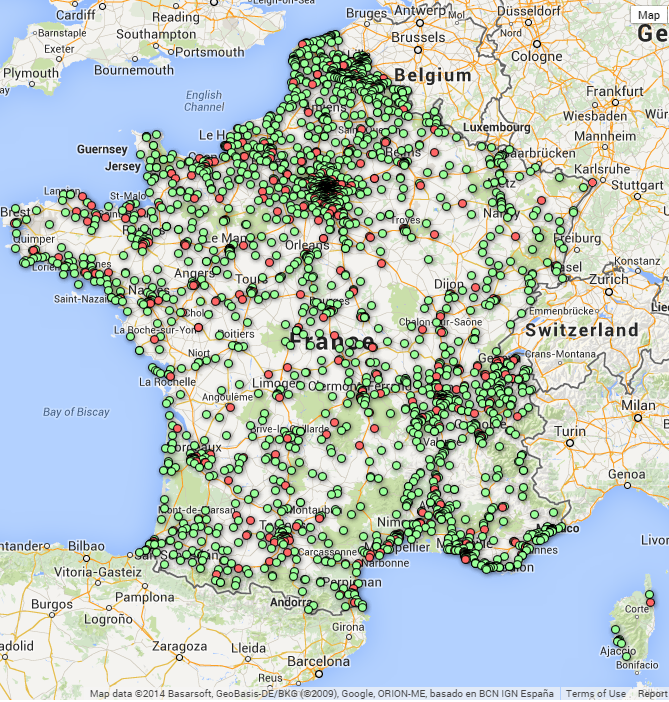
\includegraphics[width=9cm]{images/maps_group_dots/CARREFOUR.png}
        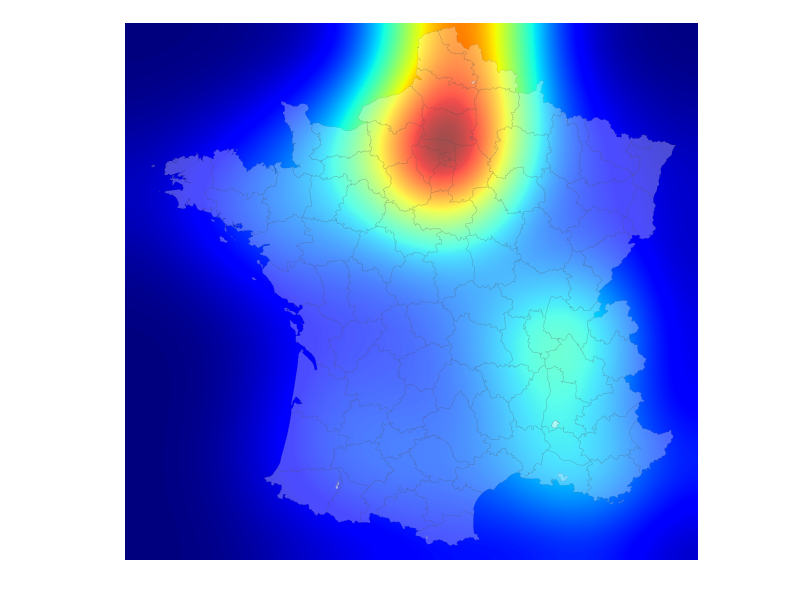
\includegraphics[width=12.8cm]{images/maps_group_heatmaps/CARREFOUR.png}
\end{figure}

\begin{figure}[H]
    \caption{CASINO}
	\centering
		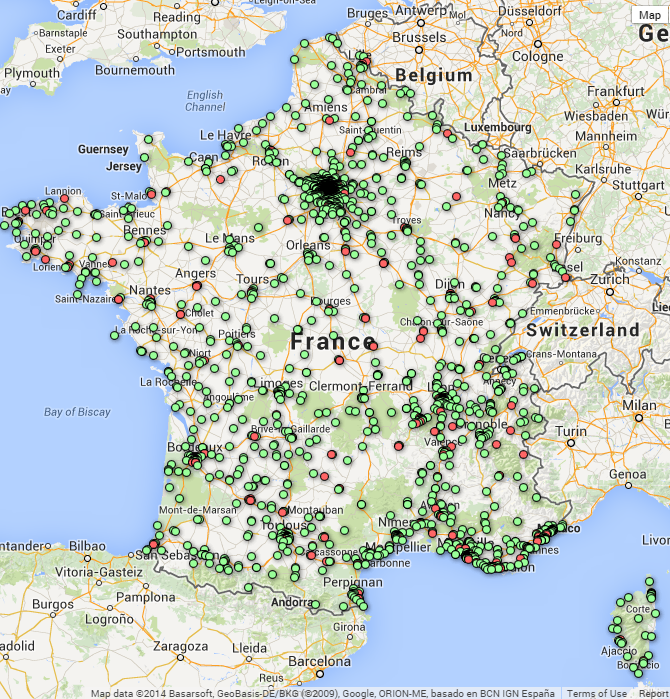
\includegraphics[width=9cm]{images/maps_group_dots/CASINO.png}
        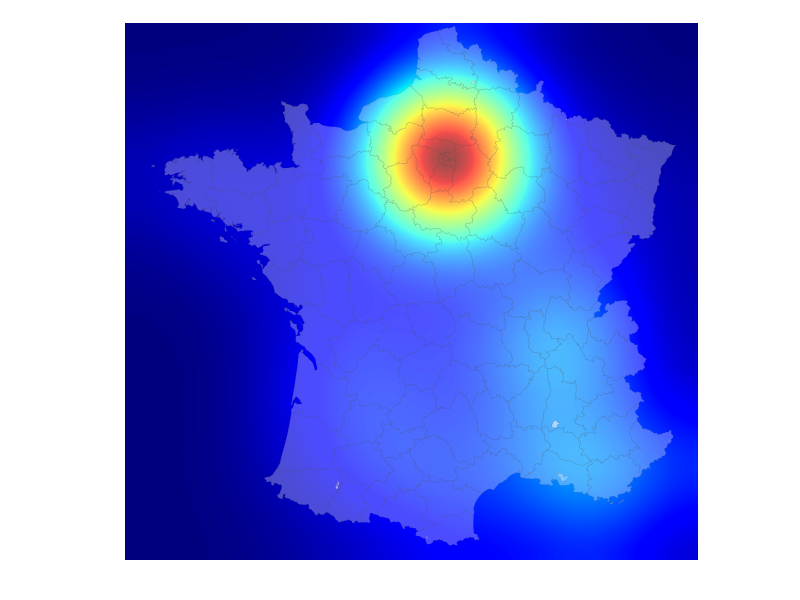
\includegraphics[width=12.8cm]{images/maps_group_heatmaps/CASINO.png}
\end{figure}

\begin{figure}[H]
    \caption{MOUSQUETAIRES}
	\centering
		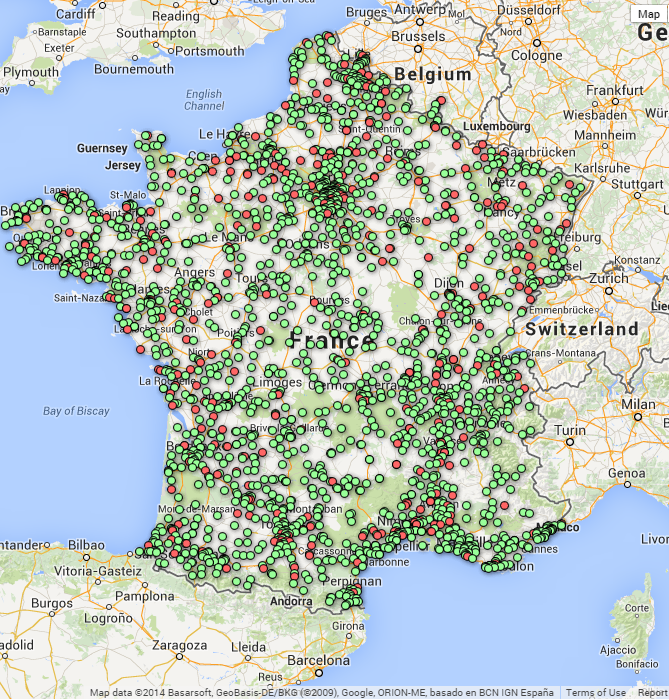
\includegraphics[width=9cm]{images/maps_group_dots/MOUSQUETAIRES.png}
        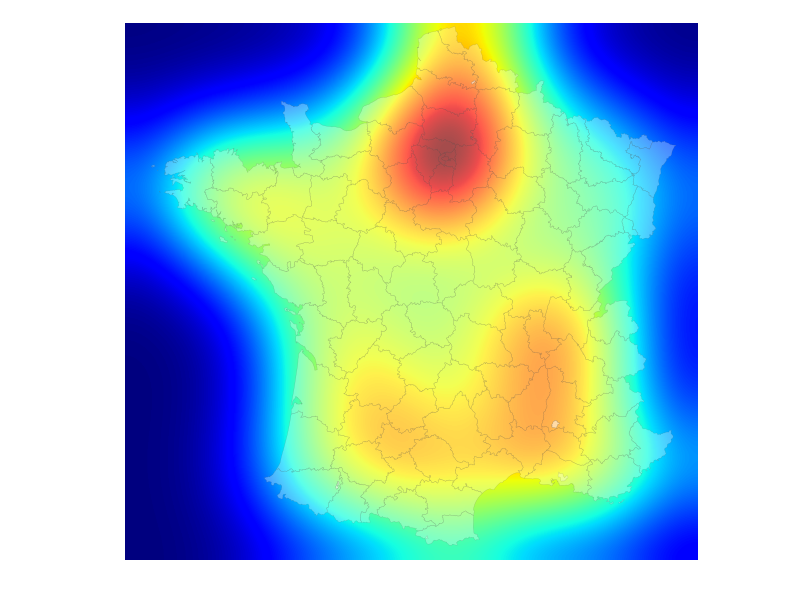
\includegraphics[width=12.8cm]{images/maps_group_heatmaps/MOUSQUETAIRES.png}
\end{figure}

\begin{figure}[H]
    \caption{LIDL}
	\centering
		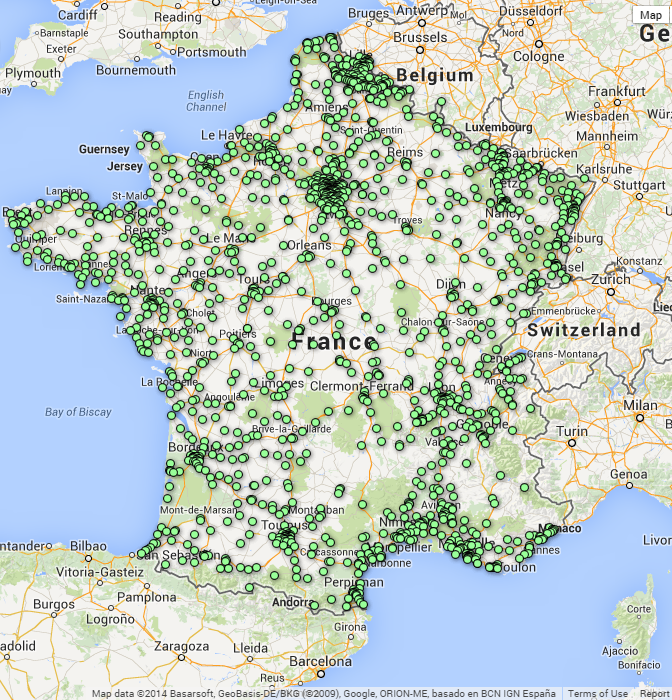
\includegraphics[width=9cm]{images/maps_group_dots/LIDL.png}
        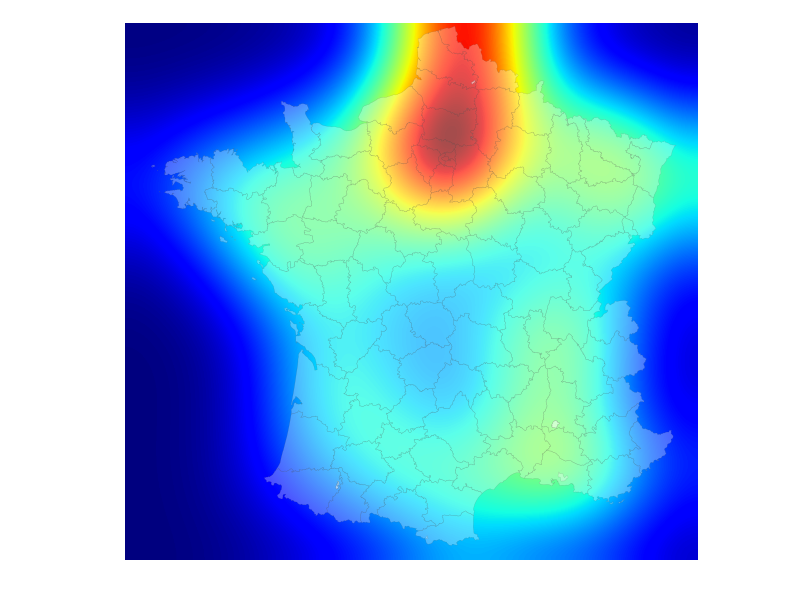
\includegraphics[width=12.8cm]{images/maps_group_heatmaps/LIDL.png}
\end{figure}

\begin{figure}[H]
    \caption{SYSTEME U}
	\centering
		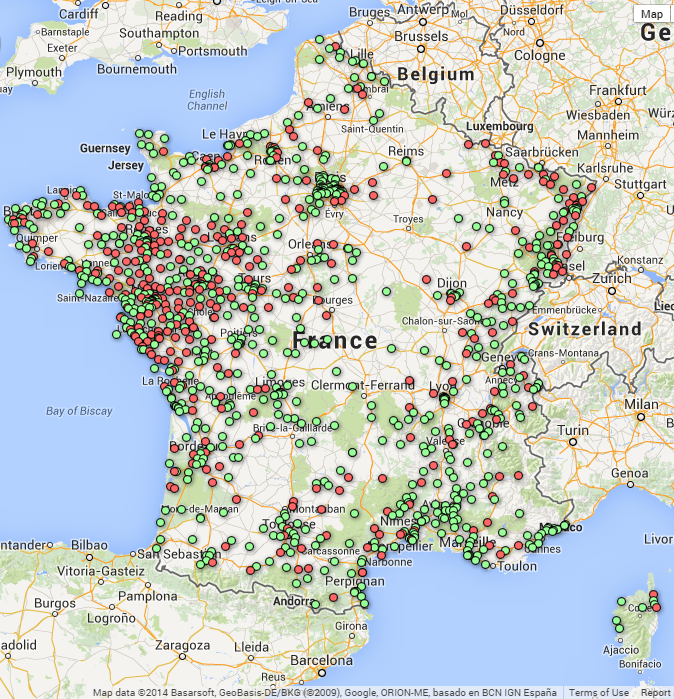
\includegraphics[width=9cm]{images/maps_group_dots/SYSTEME_U.png}
        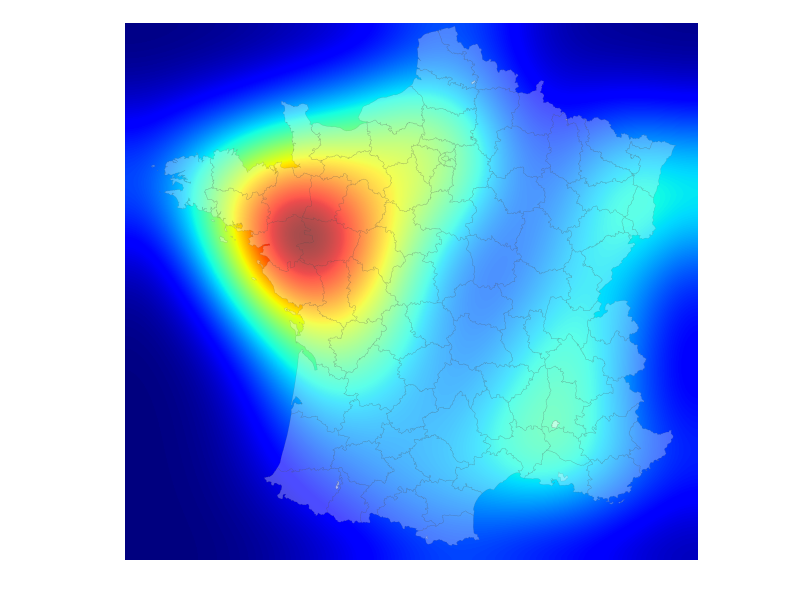
\includegraphics[width=12.8cm]{images/maps_group_heatmaps/SYSTEME_U.png}
\end{figure}

\begin{figure}[H]
    \caption{ALDI}
	\centering
		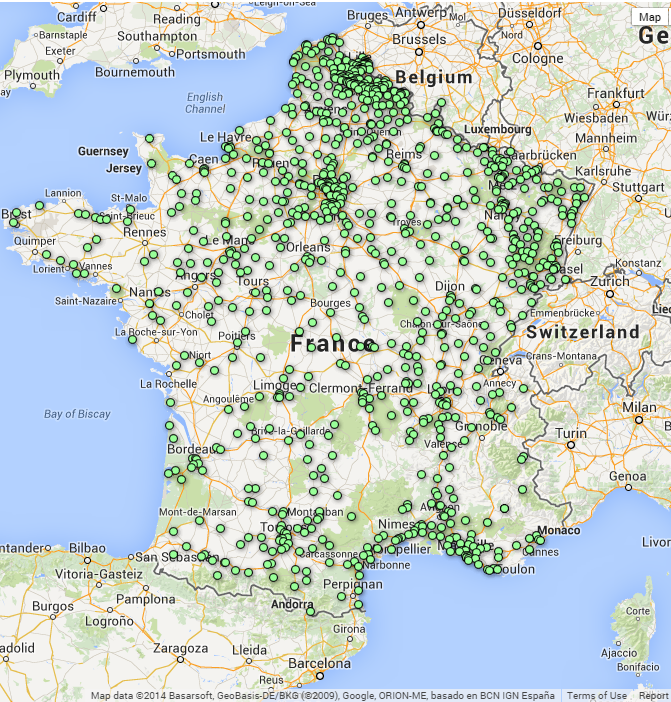
\includegraphics[width=9cm]{images/maps_group_dots/ALDI.png}
        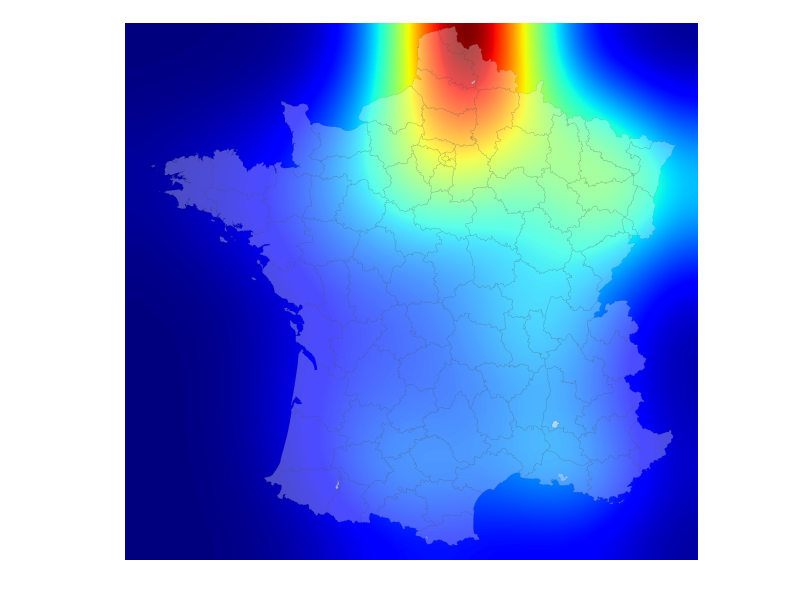
\includegraphics[width=12.8cm]{images/maps_group_heatmaps/ALDI.png}
\end{figure}

\begin{figure}[H]
    \caption{LECLERC}
	\centering
		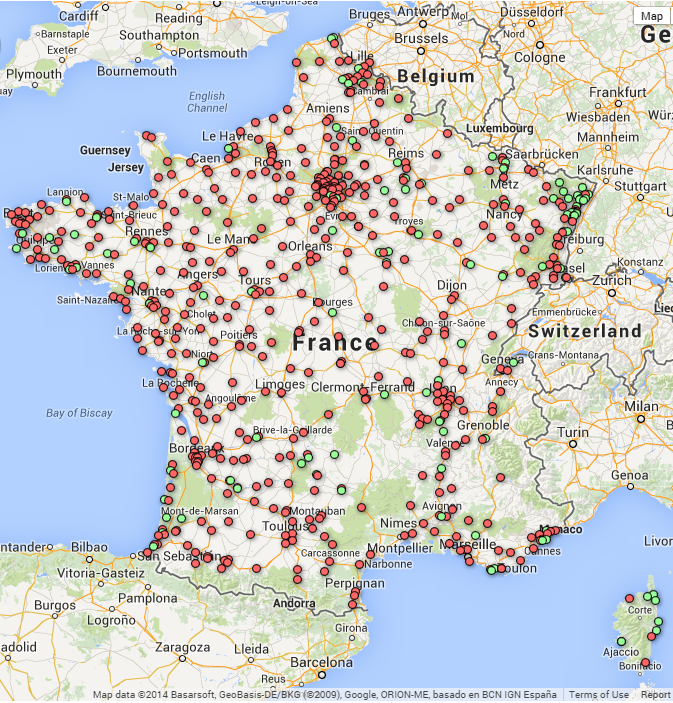
\includegraphics[width=9cm]{images/maps_group_dots/LECLERC.png}
        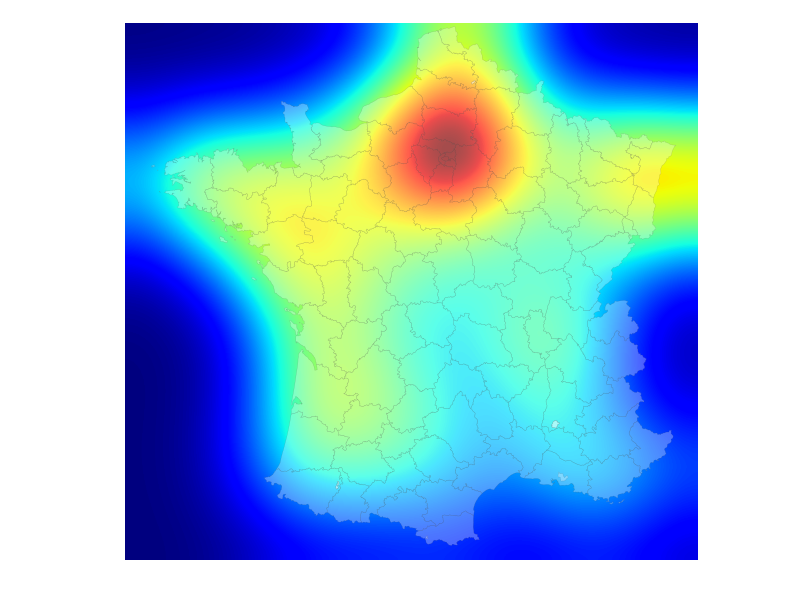
\includegraphics[width=12.8cm]{images/maps_group_heatmaps/LECLERC.png}
\end{figure}

\begin{figure}[H]
    \caption{AUCHAN}
	\centering
		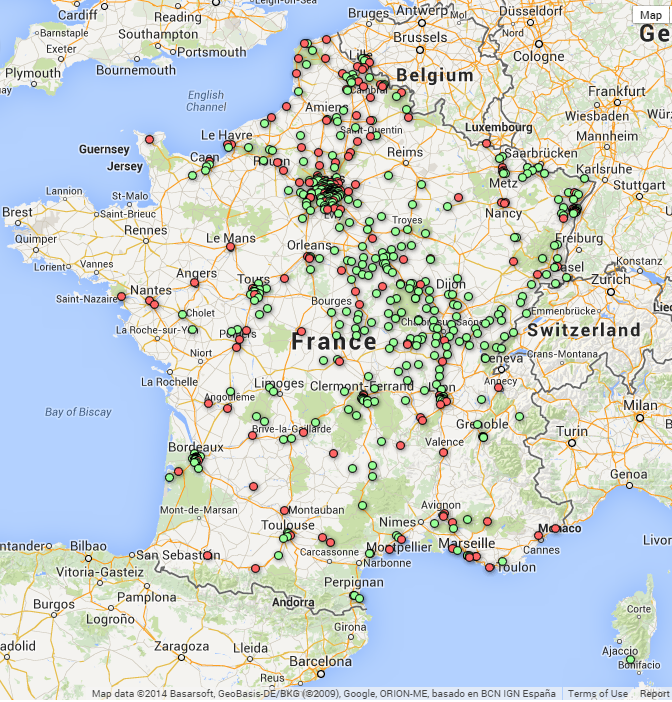
\includegraphics[width=9cm]{images/maps_group_dots/AUCHAN.png}
        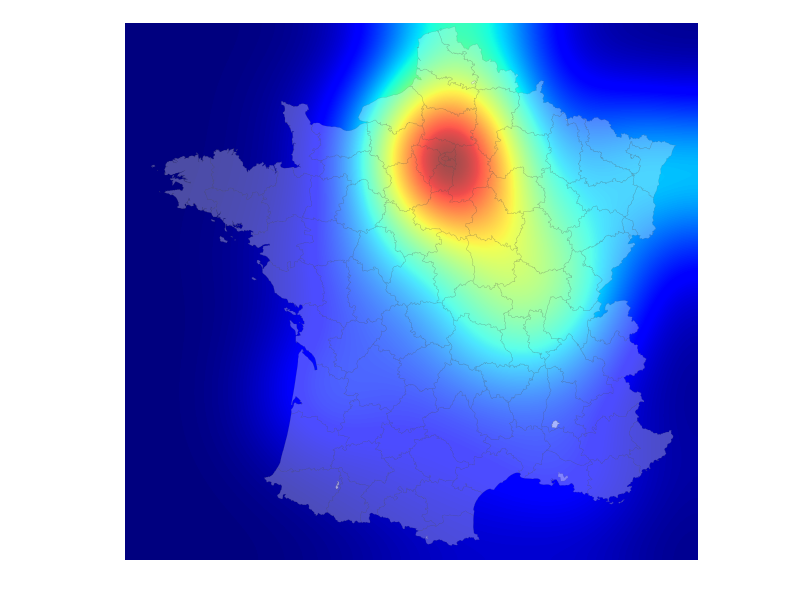
\includegraphics[width=12.8cm]{images/maps_group_heatmaps/AUCHAN.png}
\end{figure}

\begin{figure}[H]
    \caption{LOUIS DELHAIZE}
	\centering
		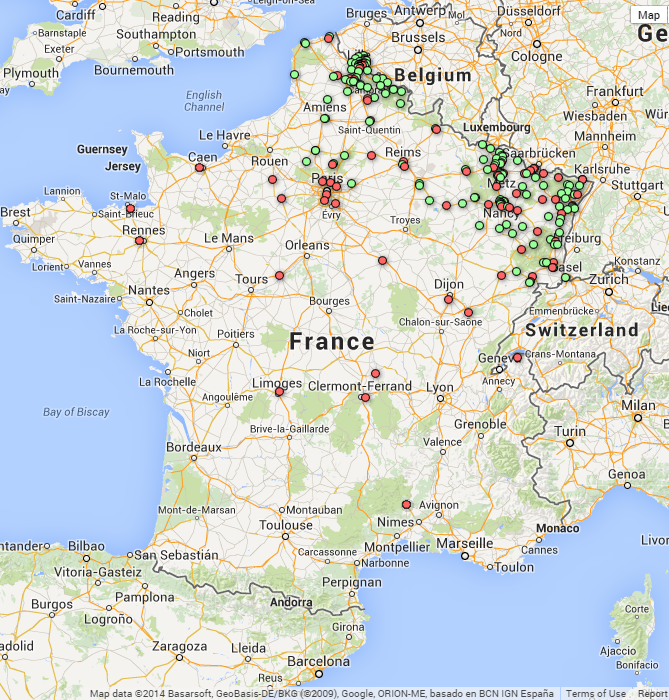
\includegraphics[width=9cm]{images/maps_group_dots/LOUIS_DELHAIZE.png}
        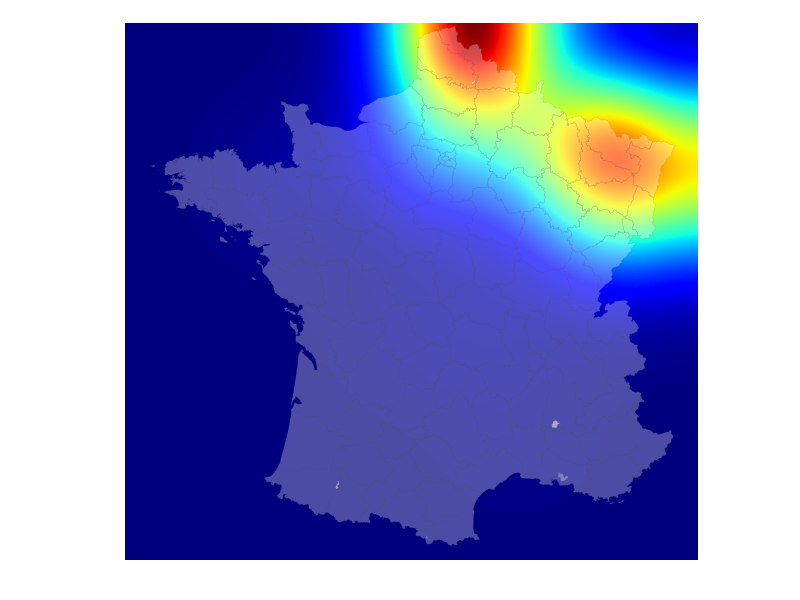
\includegraphics[width=12.8cm]{images/maps_group_heatmaps/LOUIS_DELHAIZE.png}
\end{figure}

\begin{figure}[H]
    \caption{DIAPAR}
	\centering
		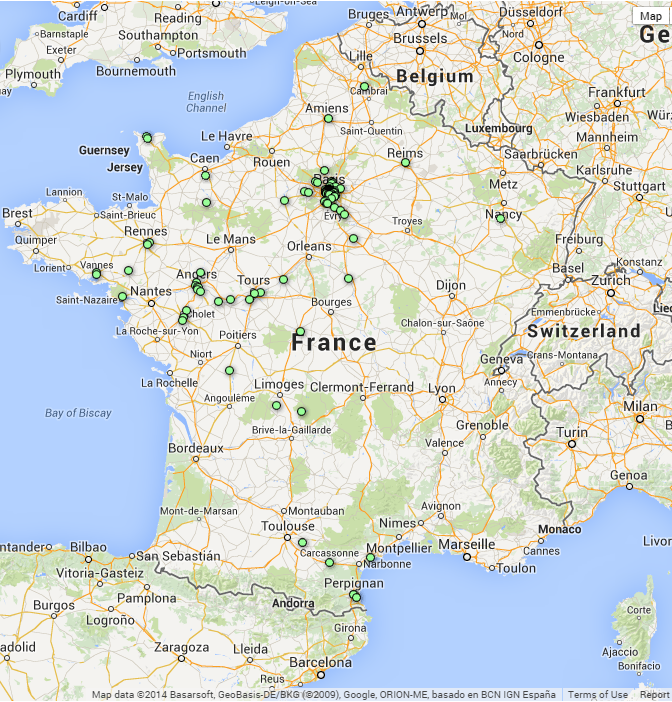
\includegraphics[width=9cm]{images/maps_group_dots/DIAPAR.png}
        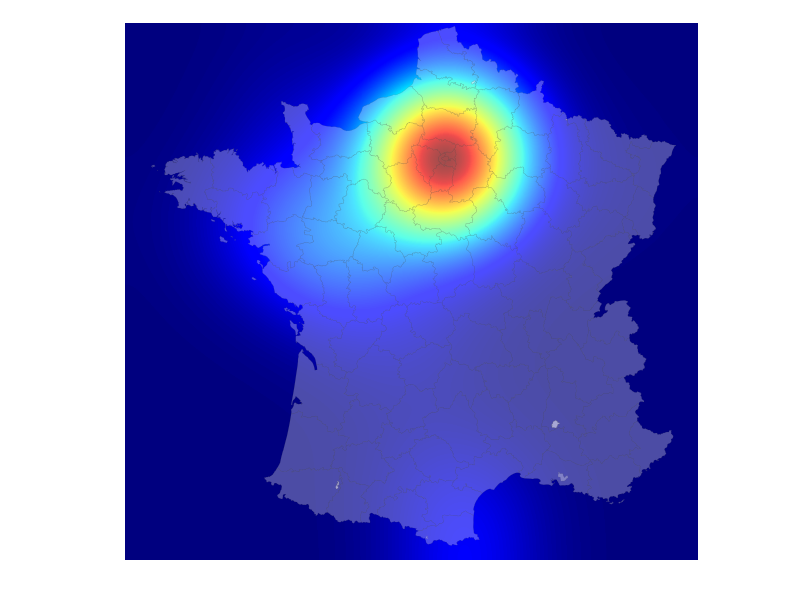
\includegraphics[width=12.8cm]{images/maps_group_heatmaps/DIAPAR.png}
\end{figure}


\begin{figure}[H]
    \caption{COLRUYT}
	\centering
		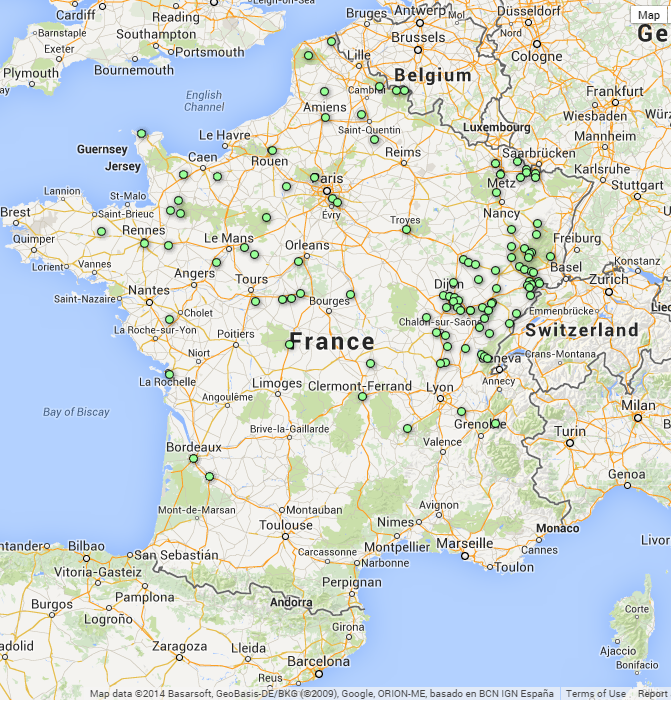
\includegraphics[width=9cm]{images/maps_group_dots/COLRUYT.png}
        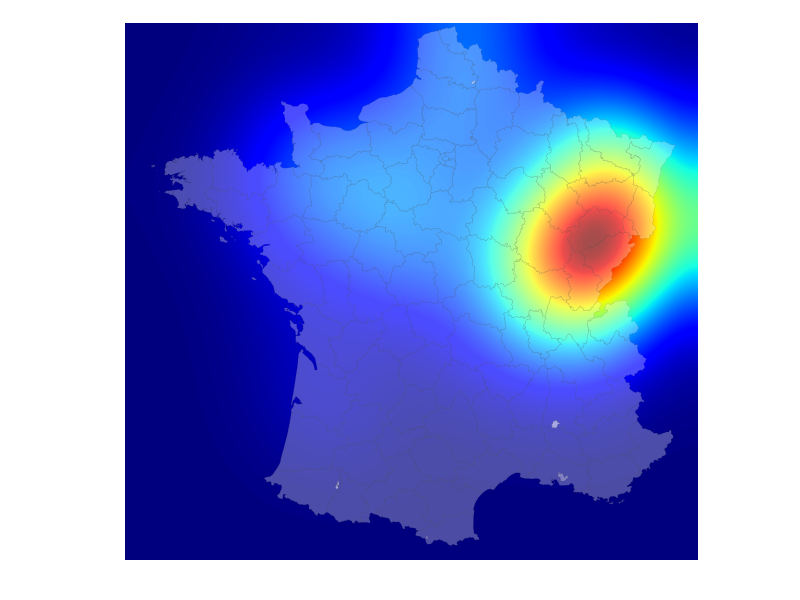
\includegraphics[width=12.8cm]{images/maps_group_heatmaps/COLRUYT.png}
\end{figure}

\begin{figure}[H]
    \caption{OTHER}
	\centering
		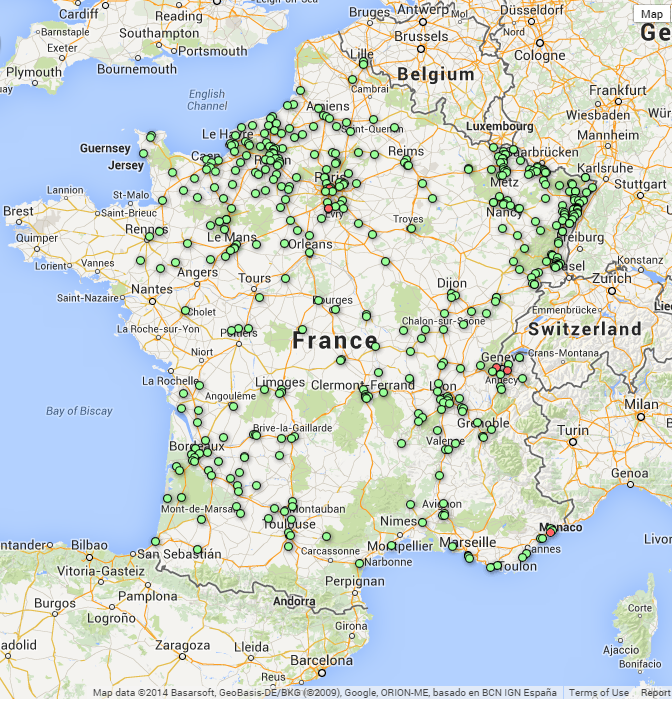
\includegraphics[width=9cm]{images/maps_group_dots/AUTRE.png}
        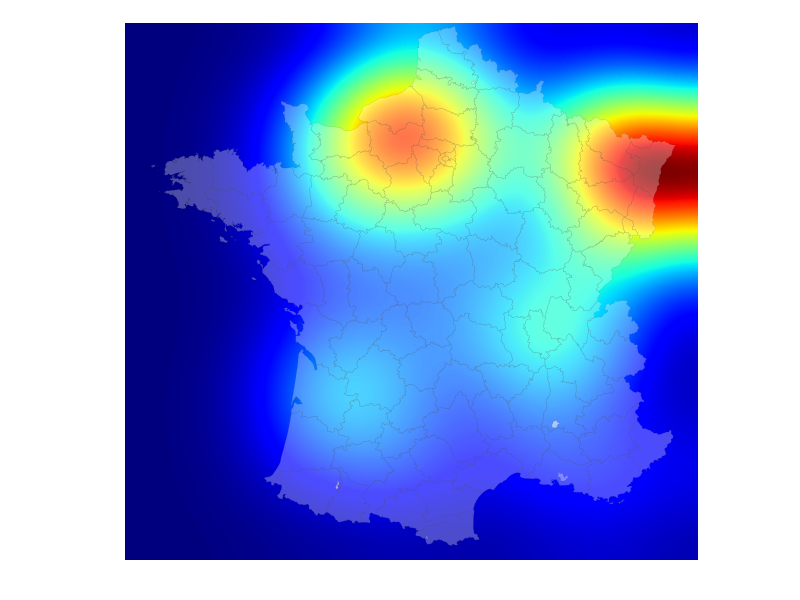
\includegraphics[width=12.8cm]{images/maps_group_heatmaps/AUTRE.png}
\end{figure}

\subsection{Competition}

\begin{figure}[H]
	\centering
		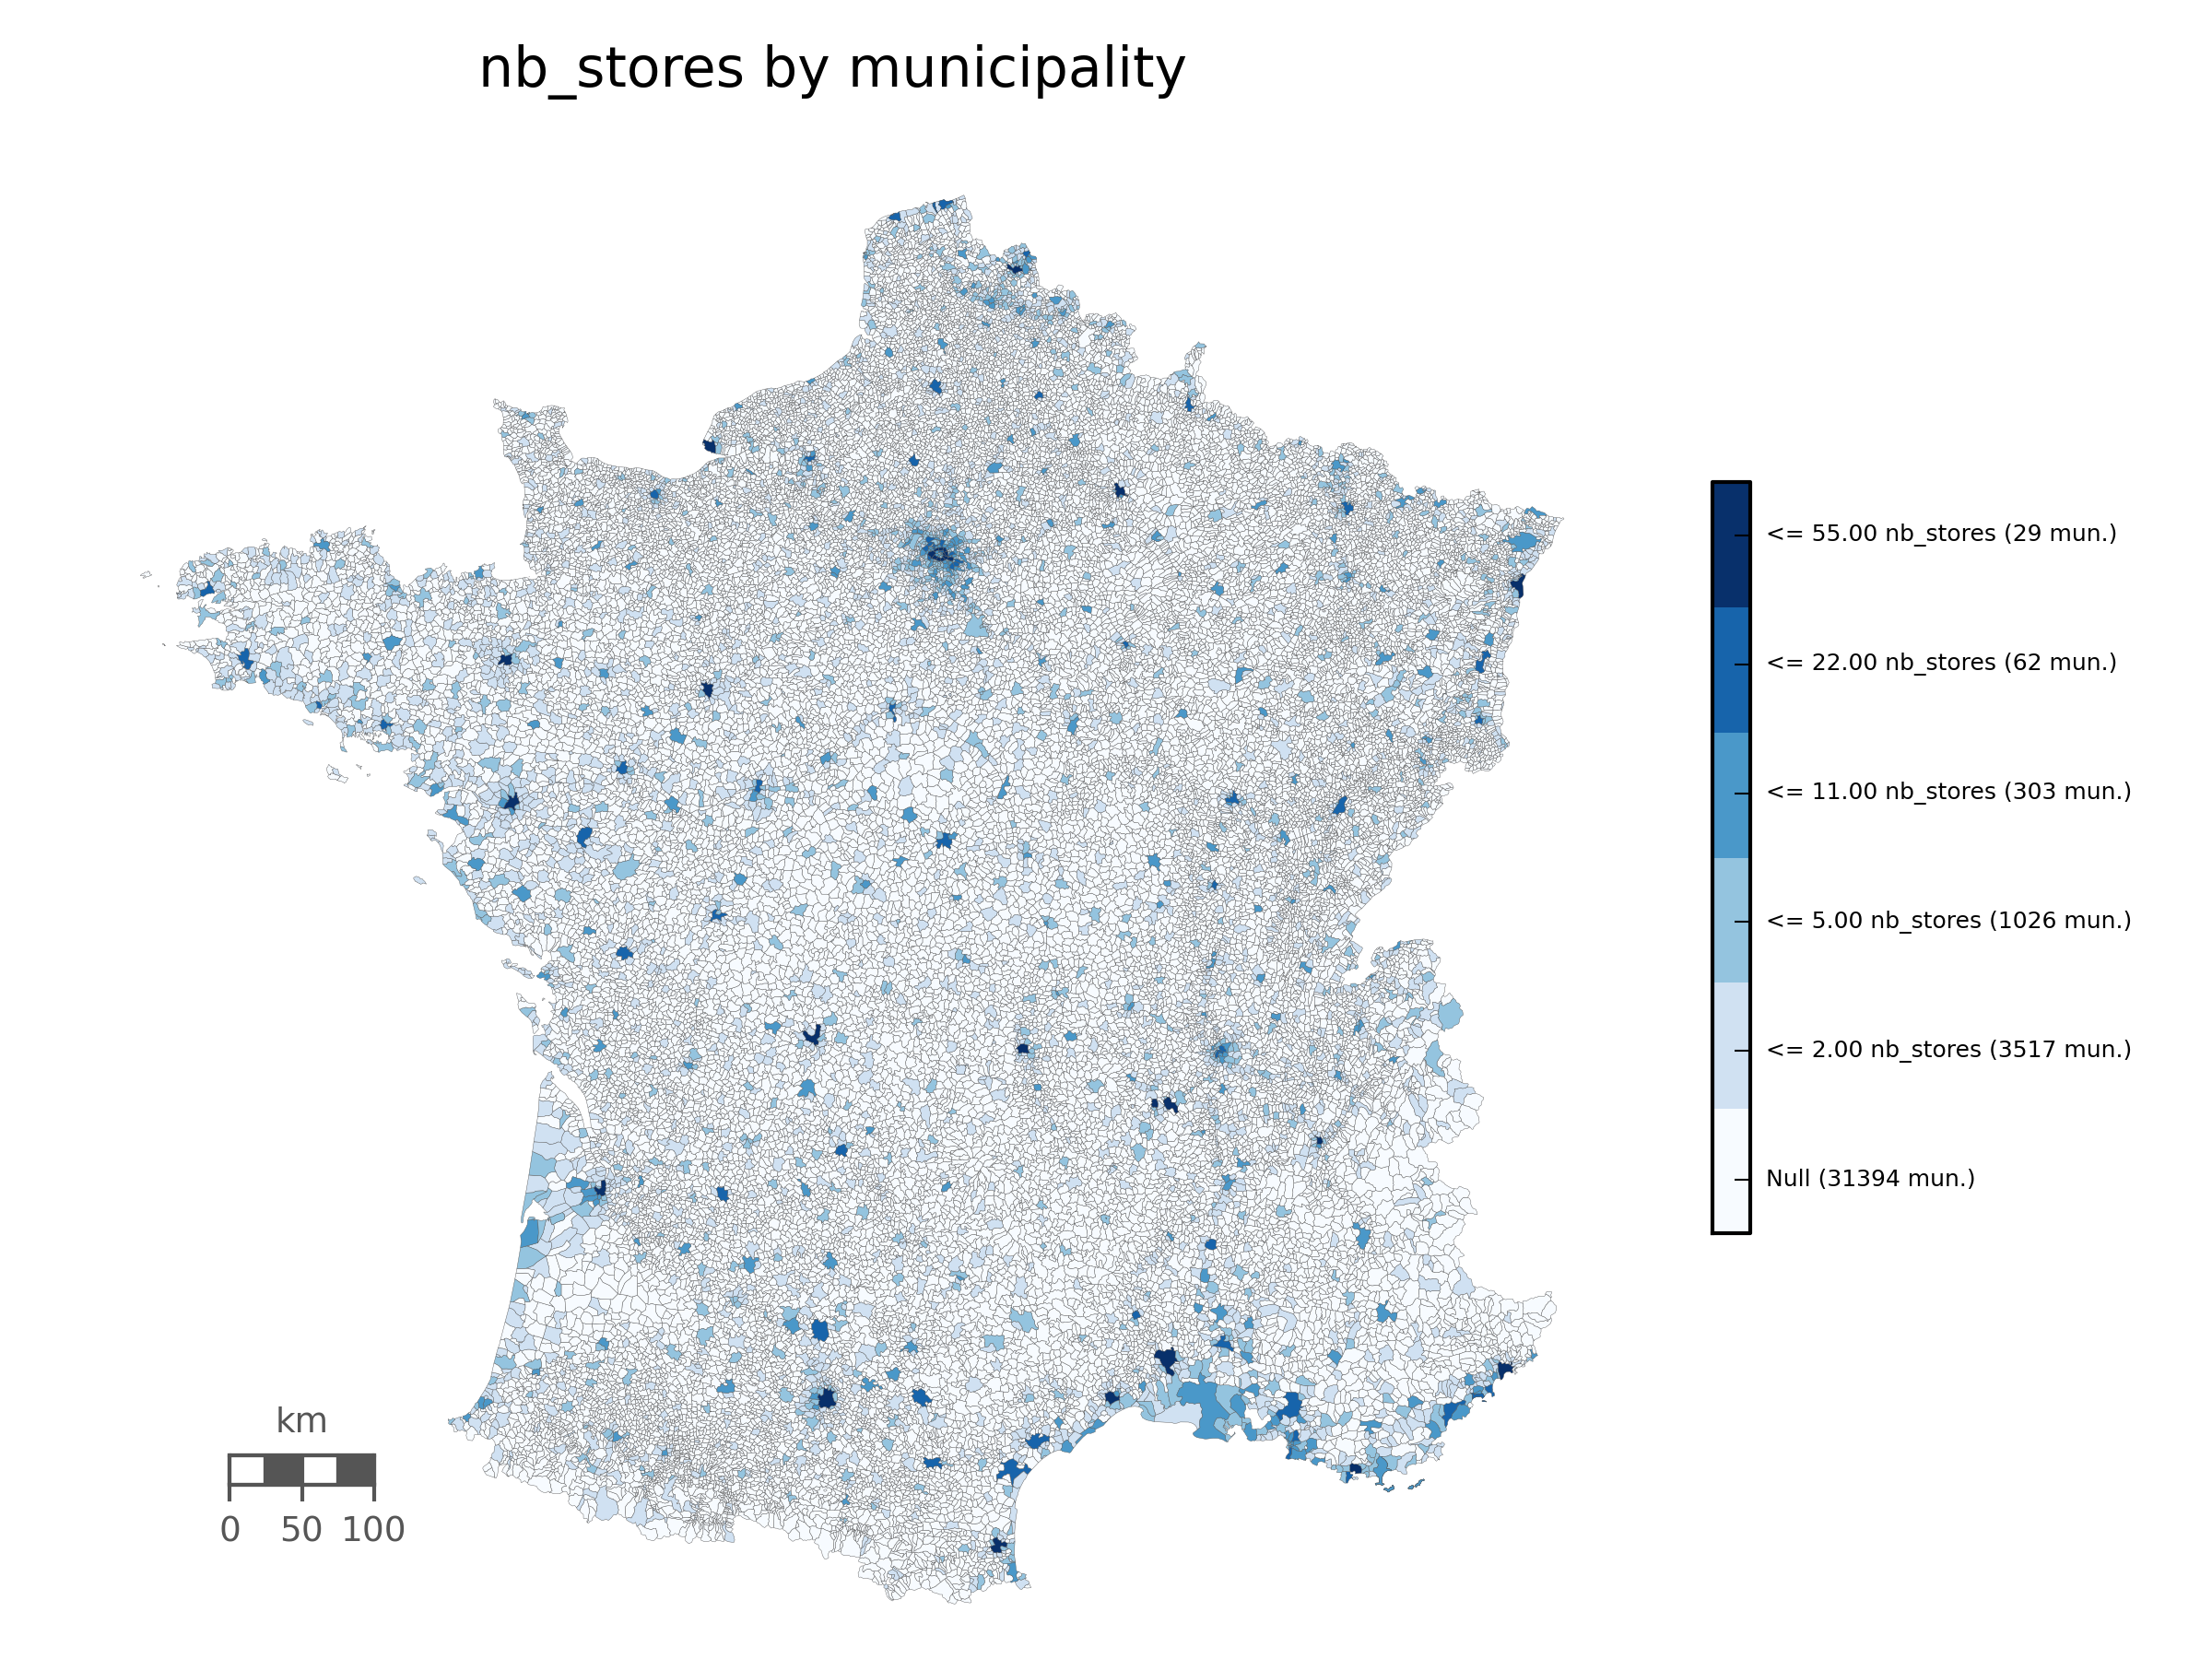
\includegraphics[width=14cm]{images/maps_competition/fra_com_nb_stores.png}
\end{figure}

\begin{figure}[H]
	\centering
		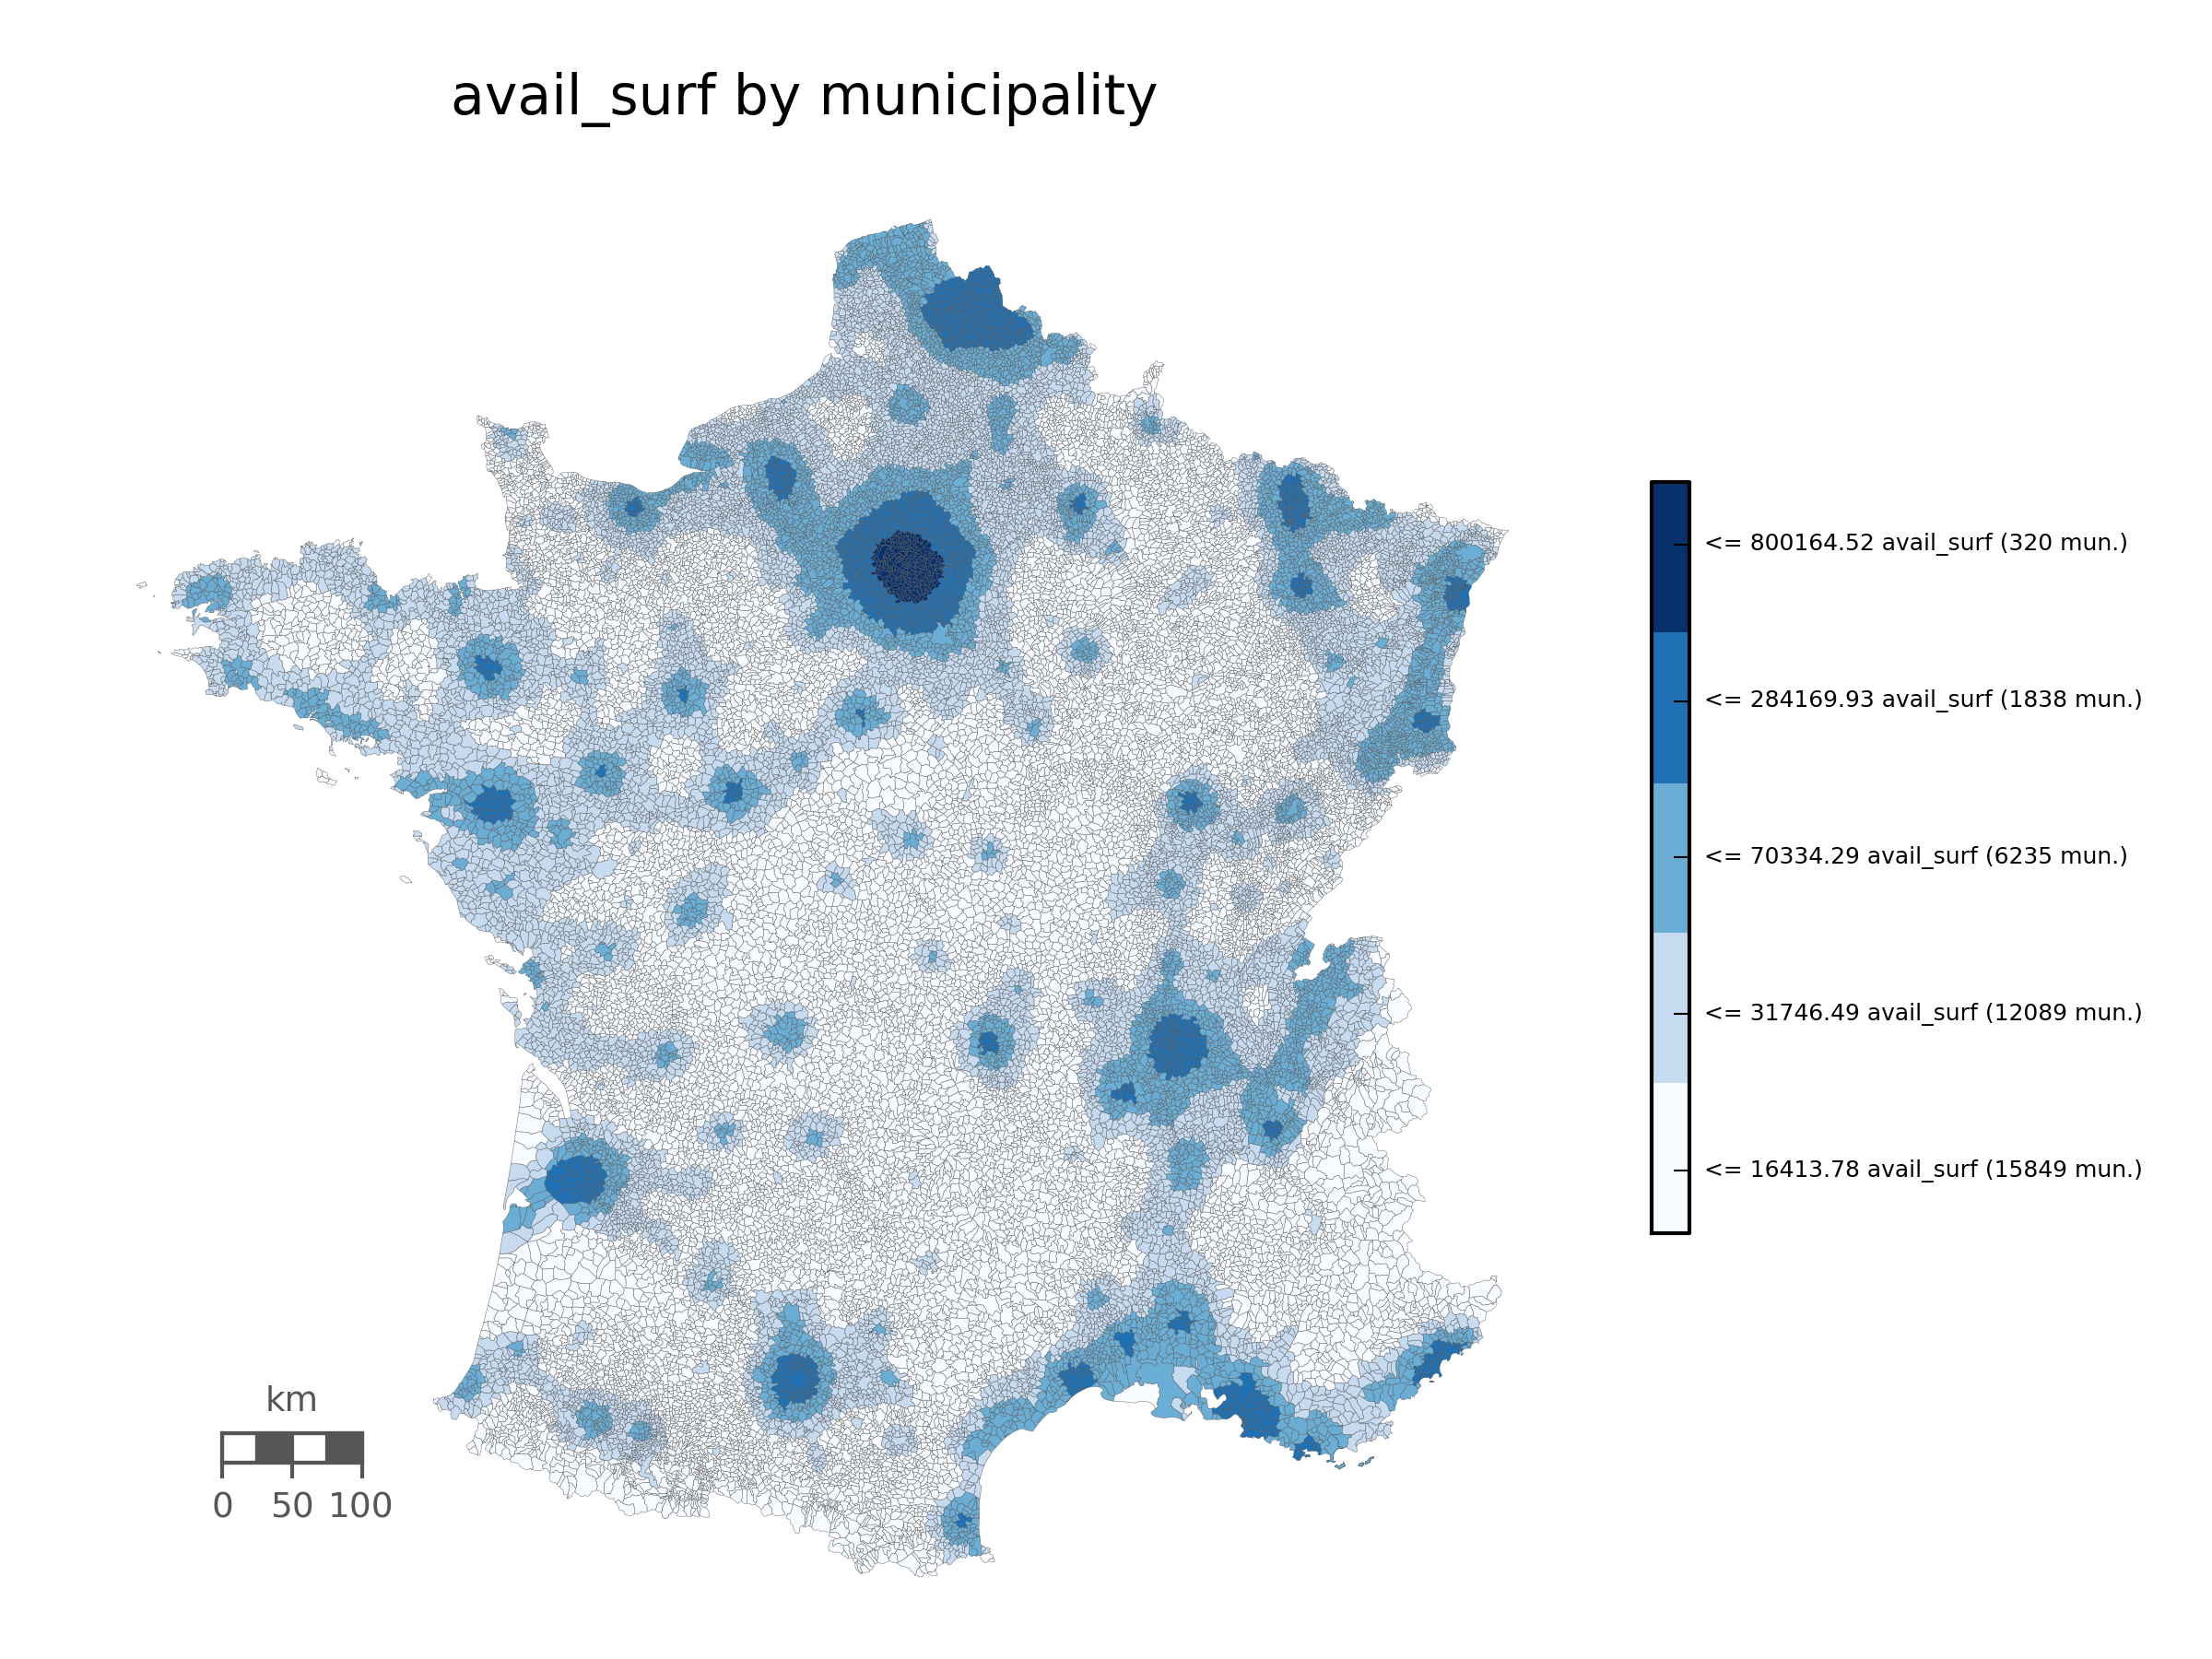
\includegraphics[width=14cm]{images/maps_competition/fra_com_avail_surf.png}
\end{figure}

\begin{figure}[H]
	\centering
		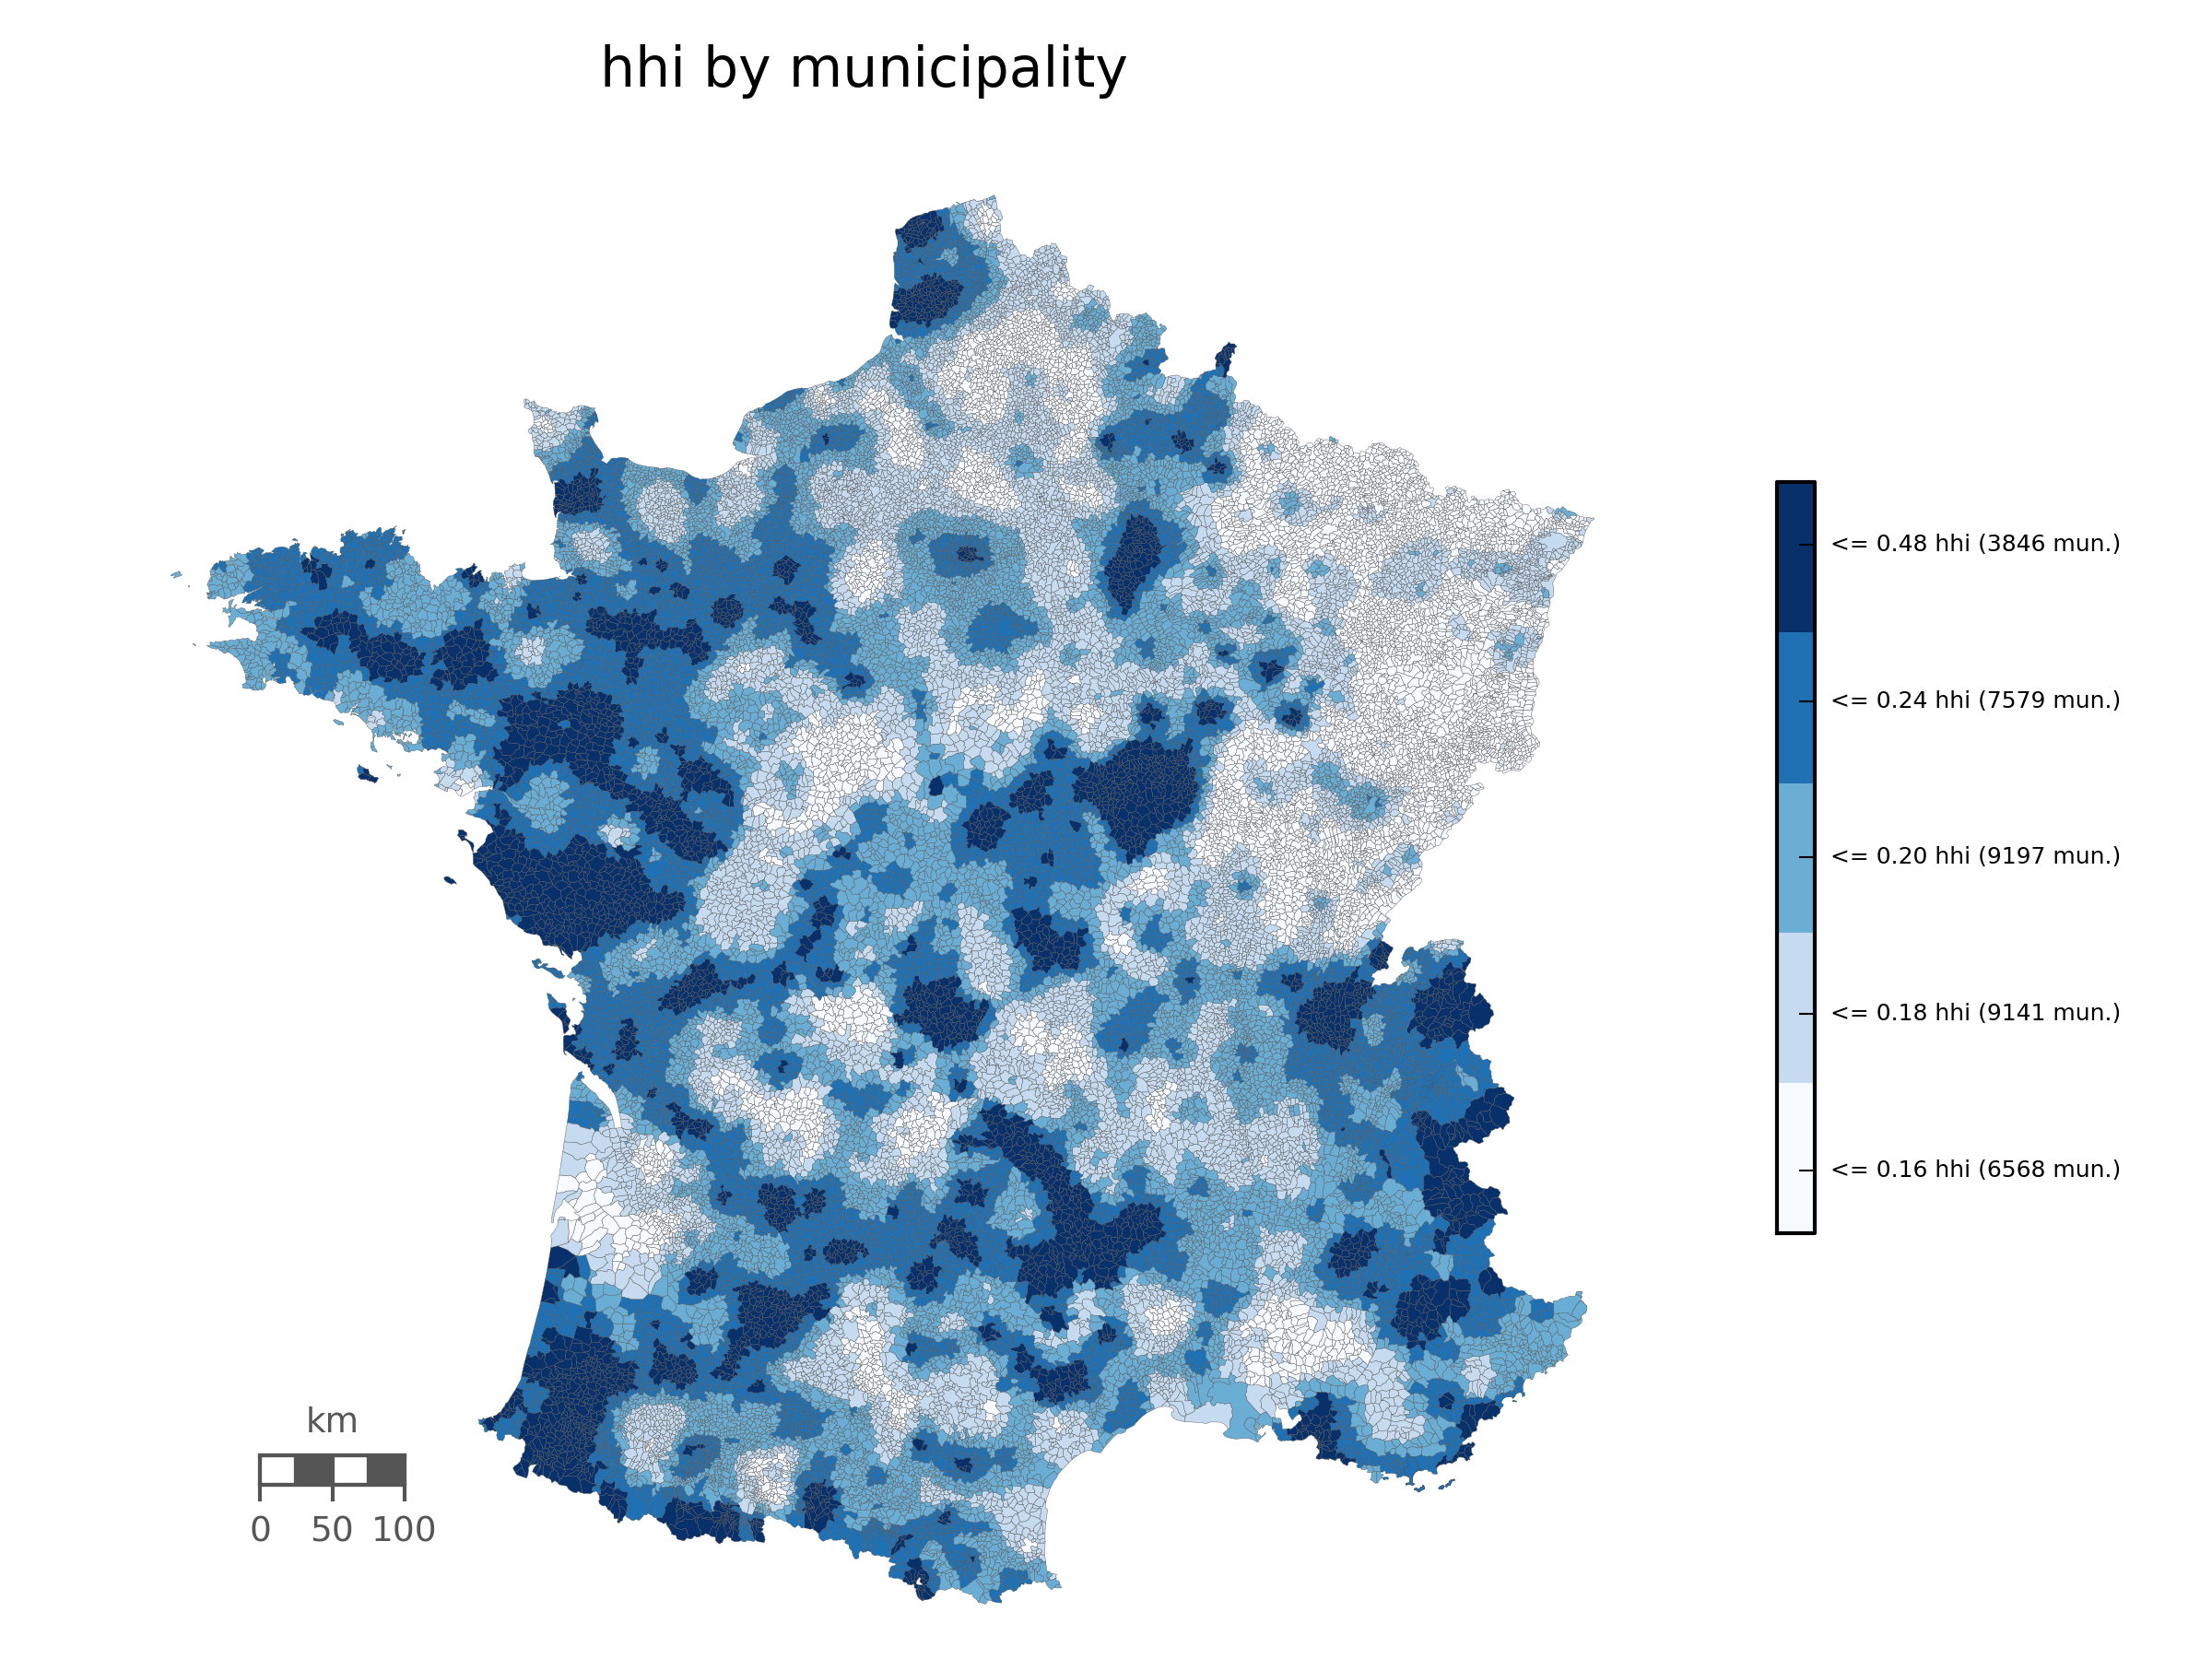
\includegraphics[width=14cm]{images/maps_competition/fra_com_hhi.png}
\end{figure}

\begin{figure}[H]
	\centering
		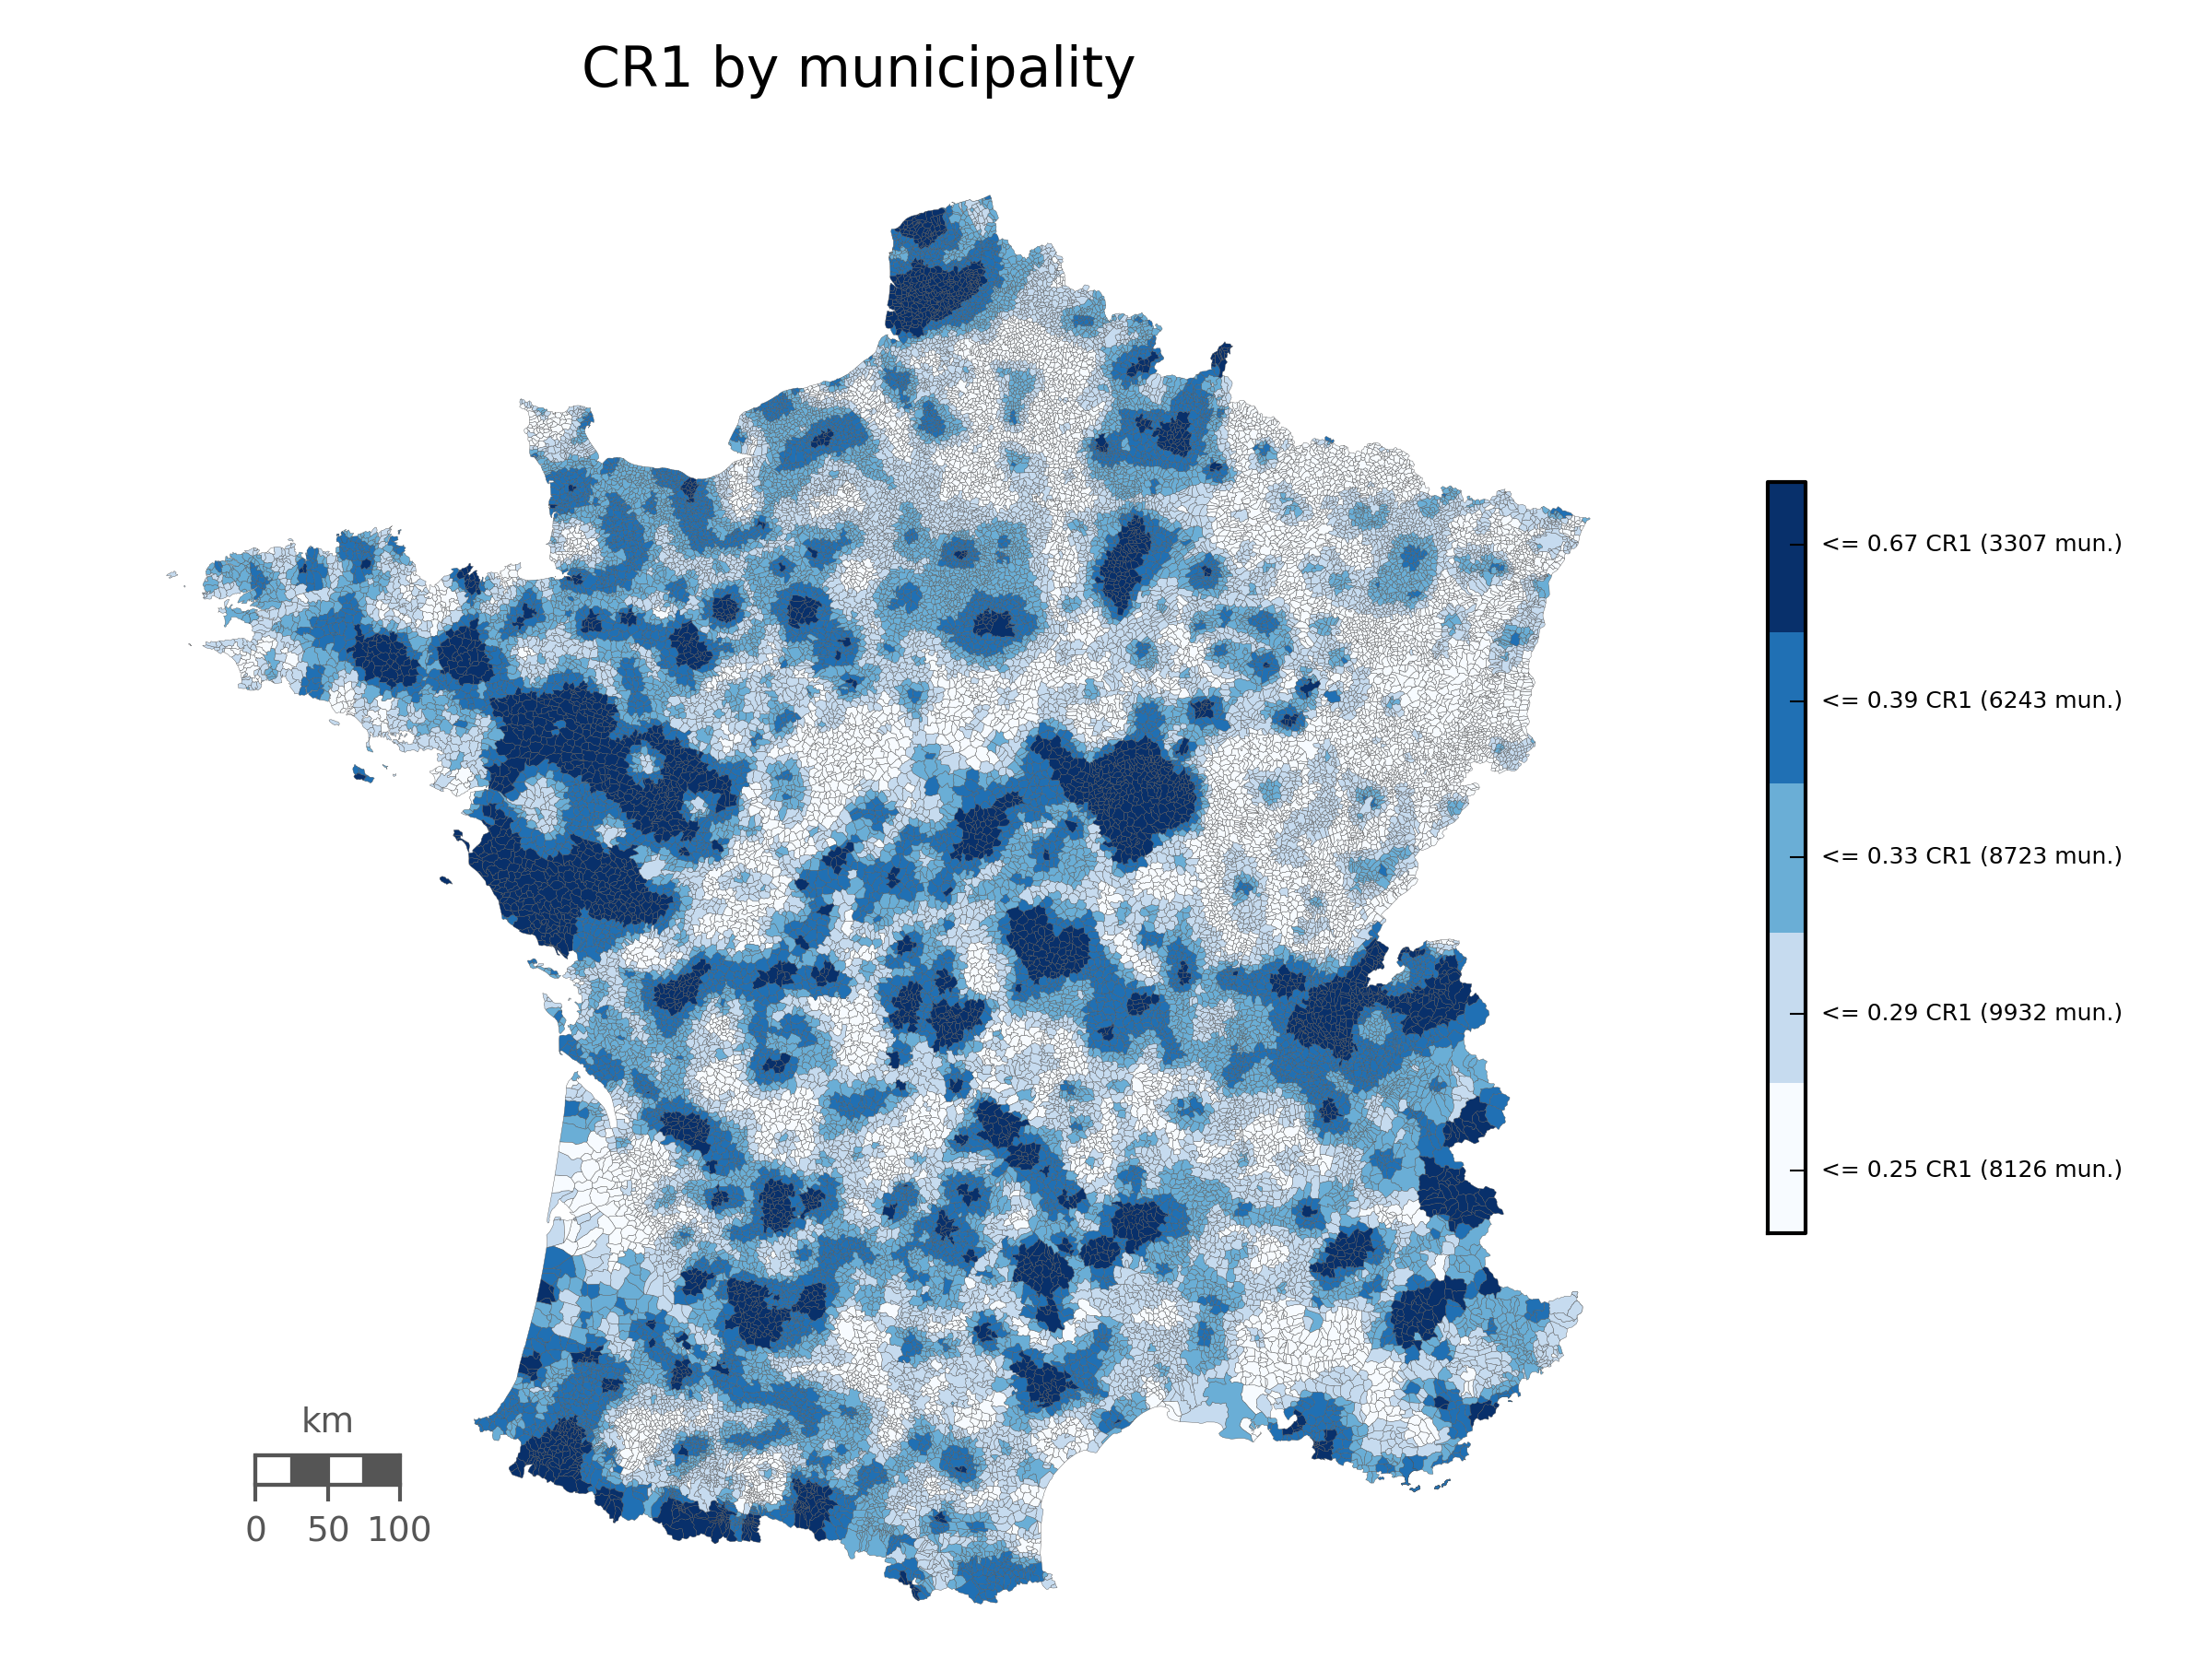
\includegraphics[width=14cm]{images/maps_competition/fra_com_CR1.png}
\end{figure}

\begin{figure}[H]
	\centering
		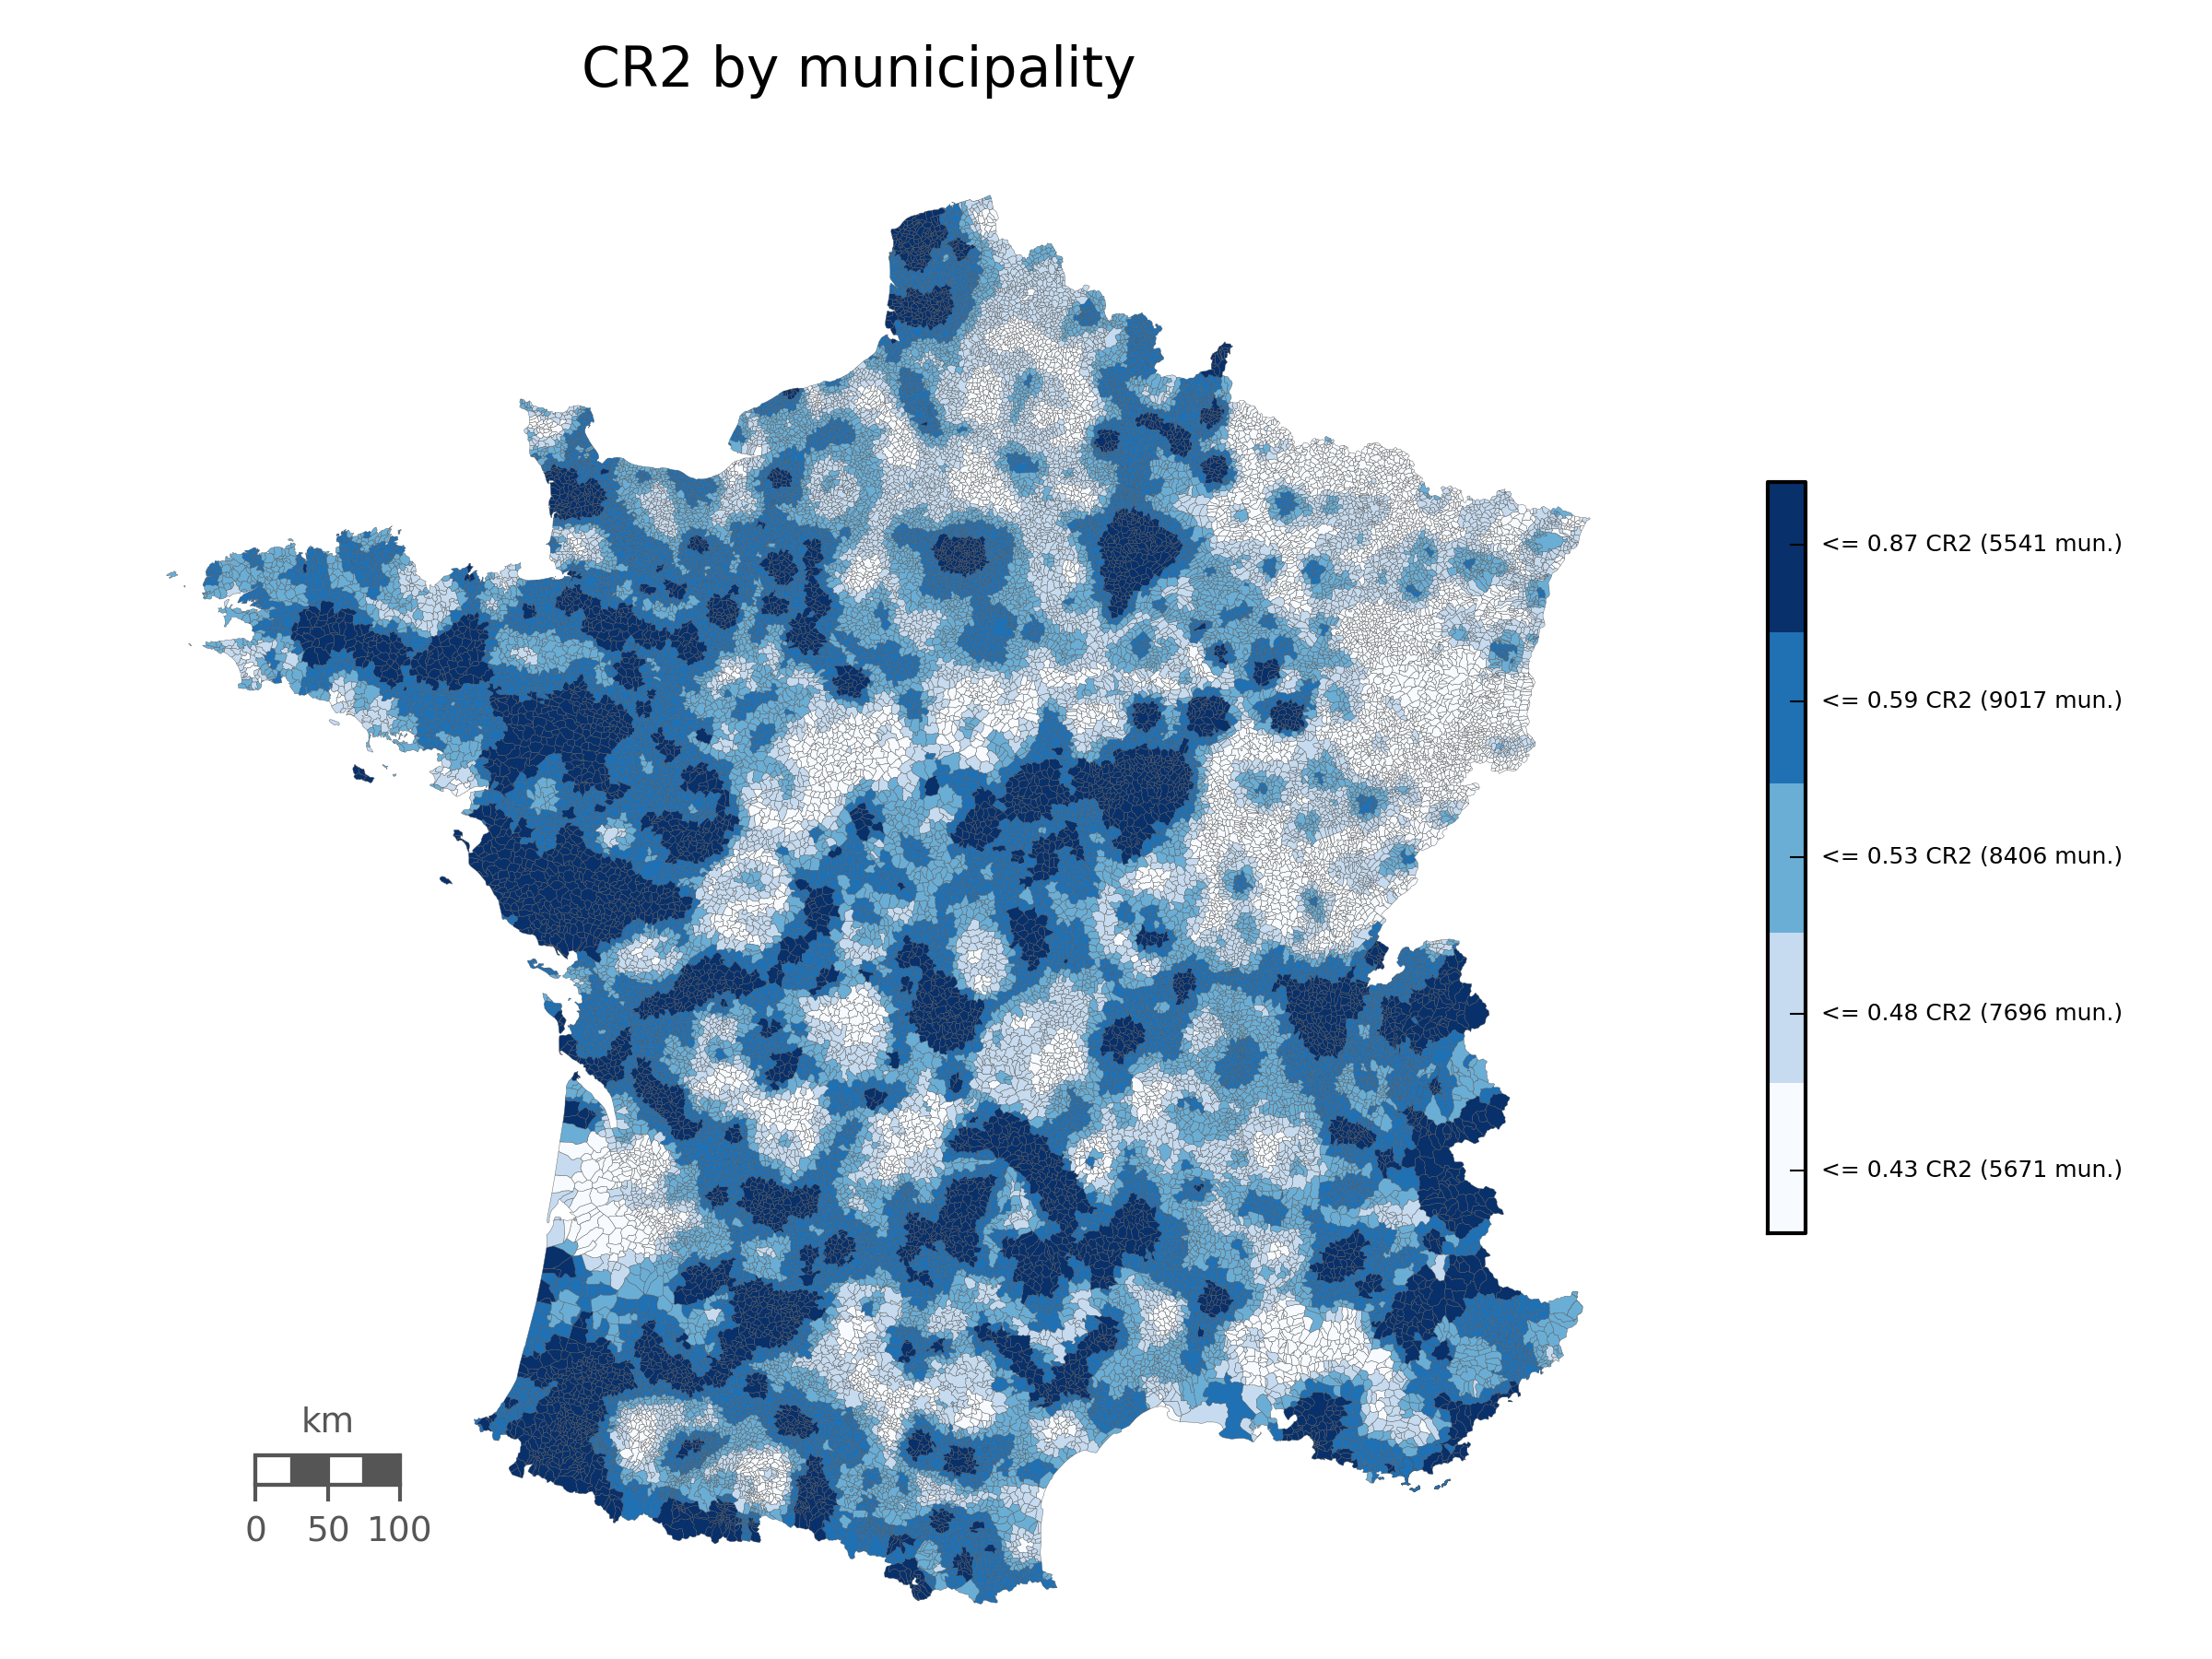
\includegraphics[width=14cm]{images/maps_competition/fra_com_CR2.png}
\end{figure}

\section{Markets}

Definition of market based on aministrative limits.

\subsection{Municipalities ("Communes")}

There are 36,208 municipalities in Metropolitan France, with a total population of 62.5 million inhabitants (Census 2010). Only 4,864 municipalities have a grocery store (hard discount or supermarket with surface above $400m^2$). This leaves 28.7\% of the population living in municipalities devoid of grocery store.

\begin{table}[H]
\caption{Top 20 "Aires urbaines" by population}
\small
%\setlength{\tabcolsep}{2pt}
\renewcommand{\arraystretch}{0.7}% Tighter

\begin{tabular}{llrrrrrr}
\toprule
Area             &      Pop   &   Size     &  Pop       & Nb         &  Pop (th)  & Cum GS          & Pop by   \\
Name             &      (th)  & (th $km^2$)&  density   & GS         &  by Nb GS  & Surf (th $m^2$) & GS $m^2$ \\
\midrule
         Paris &      2,244 &        105 &       21,289 &        459 &       4.89 &        363 &        6.18 \\
     Marseille &        851 &        241 &        3,536 &        118 &       7.21 &        204 &        4.17 \\
          Lyon &        484 &         48 &       10,118 &         70 &       6.92 &         81 &        5.98 \\
      Toulouse &        442 &        118 &        3,735 &         47 &       9.40 &         85 &        5.21 \\
          Nice &        343 &         72 &        4,773 &         55 &       6.24 &         81 &        4.22 \\
        Nantes &        285 &         65 &        4,371 &         32 &       8.91 &         66 &        4.29 \\
    Strasbourg &        272 &         78 &        3,473 &         44 &       6.18 &         59 &        4.58 \\
   Montpellier &        257 &         57 &        4,524 &         30 &       8.58 &         57 &        4.53 \\
      Bordeaux &        239 &         49 &        4,845 &         28 &       8.54 &         63 &        3.80 \\
         Lille &        228 &         35 &        6,533 &         32 &       7.11 &         59 &        3.88 \\
        Rennes &        207 &         50 &        4,111 &         26 &       7.97 &         53 &        3.92 \\
         Reims &        180 &         47 &        3,838 &         30 &       6.00 &         54 &        3.35 \\
      Le Havre &        175 &         47 &        3,738 &         24 &       7.31 &         44 &        3.96 \\
 Saint-Étienne &        171 &         80 &        2,142 &         23 &       7.45 &         40 &        4.26 \\
        Toulon &        165 &         43 &        3,841 &         23 &       7.15 &         30 &        5.43 \\
      Grenoble &        156 &         18 &        8,585 &         23 &       6.77 &         24 &        6.58 \\
         Dijon &        151 &         40 &        3,742 &         17 &       8.89 &         39 &        3.87 \\
        Angers &        148 &         43 &        3,455 &         18 &       8.20 &         55 &        2.66 \\
  Villeurbanne &        145 &         15 &        9,997 &         15 &       9.68 &         17 &        8.69 \\
       Le Mans &        143 &         53 &        2,701 &         26 &       5.49 &         54 &        2.66 \\
\bottomrule
\end{tabular}

\end{table}

\subsection{Areas in terms of urbanism ("Unites urbaines")}

Based on residential areas (c. 2300): area with no discontinuity in housing of 200m or more and more than 2000 inhabitants.

\begin{table}[H]
\caption{Top 20 "Unites urbaines" by population}
\small
%\setlength{\tabcolsep}{2pt}
\renewcommand{\arraystretch}{0.7}% Tighter

\begin{tabular}{llrrrrrrrr}
\toprule
Area             &      Pop   &   Size     &  Pop         & Med rev    & Nb         &  Pop (th)  & Cum GS          & Pop by       \\
Name             &      (th)  & (th $km^2$)&  density     & (th eur)   & GS         &  by Nb GS  & Surf (th $m^2$) & GS $m^2$  \\
\midrule
             Paris &     10,460 &      2,845 &        3,677 &      21.61 &      1,667 &       6.27 &      2,550 &        4.10 \\
   Marseille - Aix &      1,560 &      1,732 &          901 &      18.38 &        241 &       6.47 &        453 &        3.44 \\
              Lyon &      1,551 &      1,178 &        1,317 &      20.23 &        214 &       7.25 &        386 &        4.02 \\
        Lille (fr) &      1,018 &        443 &        2,301 &      17.50 &        171 &       5.96 &        342 &        2.98 \\
              Nice &        942 &        744 &        1,266 &      19.64 &        160 &       5.89 &        260 &        3.62 \\
          Toulouse &        880 &        812 &        1,084 &      21.07 &        138 &       6.37 &        305 &        2.88 \\
          Bordeaux &        843 &      1,173 &          719 &      20.59 &        132 &       6.39 &        307 &        2.75 \\
            Nantes &        591 &        538 &        1,100 &      20.51 &         81 &       7.30 &        212 &        2.79 \\
            Toulon &        558 &        764 &          730 &      19.04 &        102 &       5.47 &        181 &        3.09 \\
      Douai - Lens &        508 &        485 &        1,047 &      14.47 &        130 &       3.91 &        214 &        2.38 \\
          Grenoble &        497 &        512 &          970 &      20.38 &         74 &       6.72 &        143 &        3.47 \\
             Rouen &        464 &        453 &        1,023 &      18.46 &         89 &       5.21 &        176 &        2.63 \\
   Strasbourg (fr) &        450 &        240 &        1,873 &      18.53 &         75 &       6.00 &        130 &        3.45 \\
           Avignon &        442 &      1,369 &          323 &      17.01 &         96 &       4.61 &        172 &        2.57 \\
       Montpellier &        391 &        310 &        1,261 &      18.80 &         63 &       6.21 &        145 &        2.69 \\
     Saint-Étienne &        371 &        419 &          887 &      17.02 &         59 &       6.29 &        122 &        3.05 \\
           Béthune &        353 &        752 &          469 &      16.11 &         94 &       3.75 &        137 &        2.58 \\
             Tours &        346 &        664 &          521 &      19.48 &         64 &       5.41 &        142 &        2.43 \\
 Valenciennes (fr) &        335 &        440 &          761 &      14.25 &         78 &       4.29 &        125 &        2.69 \\
            Rennes &        311 &        284 &        1,092 &      20.62 &         47 &       6.61 &        117 &        2.65 \\
\bottomrule
\end{tabular}

\end{table}

\subsection{Areas in terms of employment ("Aires urbaines")}

Based on employment (c. 700): a pole with at least 10,000 jobs and each municipality in the pole must have at least c.40\% of its occupied inhabitants working in the pole or in municipalities attracted by the pole.

\begin{table}[H]
\caption{Top 20 "Aires urbaines" by population}
\small
%\setlength{\tabcolsep}{2pt}
\renewcommand{\arraystretch}{0.7}% Tighter

\begin{tabular}{llrrrrrrrr}
\toprule
Area             &      Pop   &   Size     &  Pop         & Med rev    & Nb         &  Pop (th)  & Cum GS          & Pop by       \\
Name             &      (th)  & (th $km^2$)&  density     & (th eur)   & GS         &  by Nb GS  & Surf (th $m^2$) & GS $m^2$  \\
\midrule
           Paris &     12,223 &     17,174 &          712 &      21.76 &      1,973 &       6.20 &      3,141 &        3.89 \\
            Lyon &      2,166 &      6,019 &          360 &      20.09 &        299 &       7.24 &        533 &        4.06 \\
 Marseille - Aix &      1,718 &      3,174 &          541 &      18.76 &        267 &       6.44 &        484 &        3.55 \\
        Toulouse &      1,232 &      5,381 &          229 &      20.73 &        208 &       5.92 &        408 &        3.02 \\
      Lille (fr) &      1,158 &        926 &        1,251 &      18.08 &        197 &       5.88 &        379 &        3.06 \\
        Bordeaux &      1,128 &      5,613 &          201 &      20.13 &        190 &       5.94 &        404 &        2.79 \\
            Nice &      1,001 &      2,585 &          387 &      19.64 &        165 &       6.07 &        267 &        3.75 \\
          Nantes &        873 &      3,302 &          264 &      19.93 &        119 &       7.34 &        291 &        3.00 \\
 Strasbourg (fr) &        761 &      2,198 &          346 &      20.07 &        140 &       5.44 &        248 &        3.07 \\
        Grenoble &        670 &      2,621 &          255 &      20.69 &         97 &       6.90 &        179 &        3.75 \\
          Rennes &        672 &      3,747 &          179 &      19.84 &        109 &       6.16 &        223 &        3.02 \\
           Rouen &        653 &      2,367 &          276 &      19.07 &        115 &       5.68 &        218 &        3.00 \\
          Toulon &        607 &      1,196 &          508 &      19.09 &        112 &       5.42 &        196 &        3.10 \\
    Douai - Lens &        543 &        679 &          800 &      14.77 &        134 &       4.05 &        217 &        2.50 \\
     Montpellier &        549 &      1,673 &          328 &      19.18 &         81 &       6.78 &        173 &        3.17 \\
         Avignon &        511 &      2,083 &          245 &      17.28 &        104 &       4.92 &        179 &        2.85 \\
   Saint-Étienne &        509 &      1,689 &          301 &      17.69 &         77 &       6.61 &        150 &        3.39 \\
           Tours &        477 &      3,184 &          150 &      19.44 &         84 &       5.68 &        172 &        2.77 \\
   Clermont-Fer. &        464 &      2,420 &          192 &      19.76 &         83 &       5.59 &        162 &        2.87 \\
           Nancy &        435 &      2,367 &          184 &      19.62 &         79 &       5.51 &        152 &        2.85 \\
\bottomrule
\end{tabular}

\end{table}

\clearpage

\appendix

\section{"Drive-through"}

\begin{table}[H]
\caption{Drive: Surface in $m^2$ by type}
\small

\begin{tabular}{lrrrrrrrrr}
\toprule
{} &     \#Total &    \#Avail. &        Min &        Q05 &        Med &        Avg &        Q95 &        Max &        Cum \\
\midrule
Drive in &      2,046 &        247 &         10 &         54 &      1,500 &      1,395 &      2,500 &      3,900 &    344,576 \\
Drive    &        435 &        435 &        100 &        555 &      1,800 &      1,801 &      3,000 &      7,500 &    783,614 \\
All      &      2,481 &        682 &         10 &        252 &      1,600 &      1,654 &      2,897 &      7,500 &  1,128,190 \\
\bottomrule
\end{tabular}

\end{table}

\end{document}
